\chapter{Experimental Setup} % Main chapter title

\label{Chapter3} % For referencing the chapter elsewhere, use \ref{Chapter3} 

%----------------------------------------------------------------------------------------
\section{Software}
\subsection{Matlab, portaudio, playrec}{}
\label{subsec:matlab}

The main piece of software used to performed all the required measurements and experiments was Matlab, a graphical environment for the development of highly specialized and computationally intensive computer programs. Its proprietary programming language was used to design the algorithms subject of the thesis and to interact with the hardware used for the experiments, thanks to two third-party interfaces Portaudio and Playrec.
\\
In order to send the input signal to the DAC and subsequently to the Loudspeakers it was necessary to use some drivers that allowed for a low latency streaming on multiple channels. For this purpose the out-of-the-shelf package of choice were Portaudio, an open-source audio I/O library and Playrec, a middleware that builds on top of Portaudio and provides a very simple API to the Matlab environment allowing to perform non-blocking calls to the soundcard using the ASIO protocol, which allowed to satisfy the low latency communication requirements between the software and the soundcard hardware.
\\
The reason why Playrec's API were chosen among other candidates was that it allows for the simultaneous playback and recording of sound. This simplifies the IR estimation of the system. Making sure the starting sample is the same between playing and recording makes possible to have a good estimation of the acoustic delay, that is the time (expressed in number of samples) between the moment the speakers start playing, from the time the microphones start picking up the first samples of the signal.

\subsection{Logsweep signal}{}
\label{sec:logsweep}

In section \ref{subsec:greenfct} it was explained how the propagation of a soundwave can be approximated by using of the Green's Function. It was also explained that this model shows its limits when the frequency (and therefore the wavelength) of the sound signal is high enough so that the propagation field is not spherical anymore and the sound source cannot be considered as a point. Also, the presence of reflections complicates the propagation model so much, that the Green's function does not have a closed-form solution anymore and an experimental approach becomes by far the easiest way of estimating the system IR.
\\ 
In order to refine the IR estimation (which, as explained in section \ref{sec:intro} describes the characteristics of the room-speakers-microphones system), a new model is required. The function that allows for such a precise estimation is the Logsweep function, also called chirp tone.
\\
Suppose one wants to estimate the performance of a system using a sine wave. It is well known that the system response can be expressed by the formula
\begin{equation}
h(t) = \frac{y(t)}{x(t)}
\label{eqn:h}
\end{equation}

Where $x(t)$ is the input signal and $y(t)$ is the output. The frequency response of a real loudspeaker system, excited with a sine wave at a specific frequency ($200$Hz), that is obtained by Fourier transforming $h(t)$ looks similar to 
\begin{figure}[th]
\centering
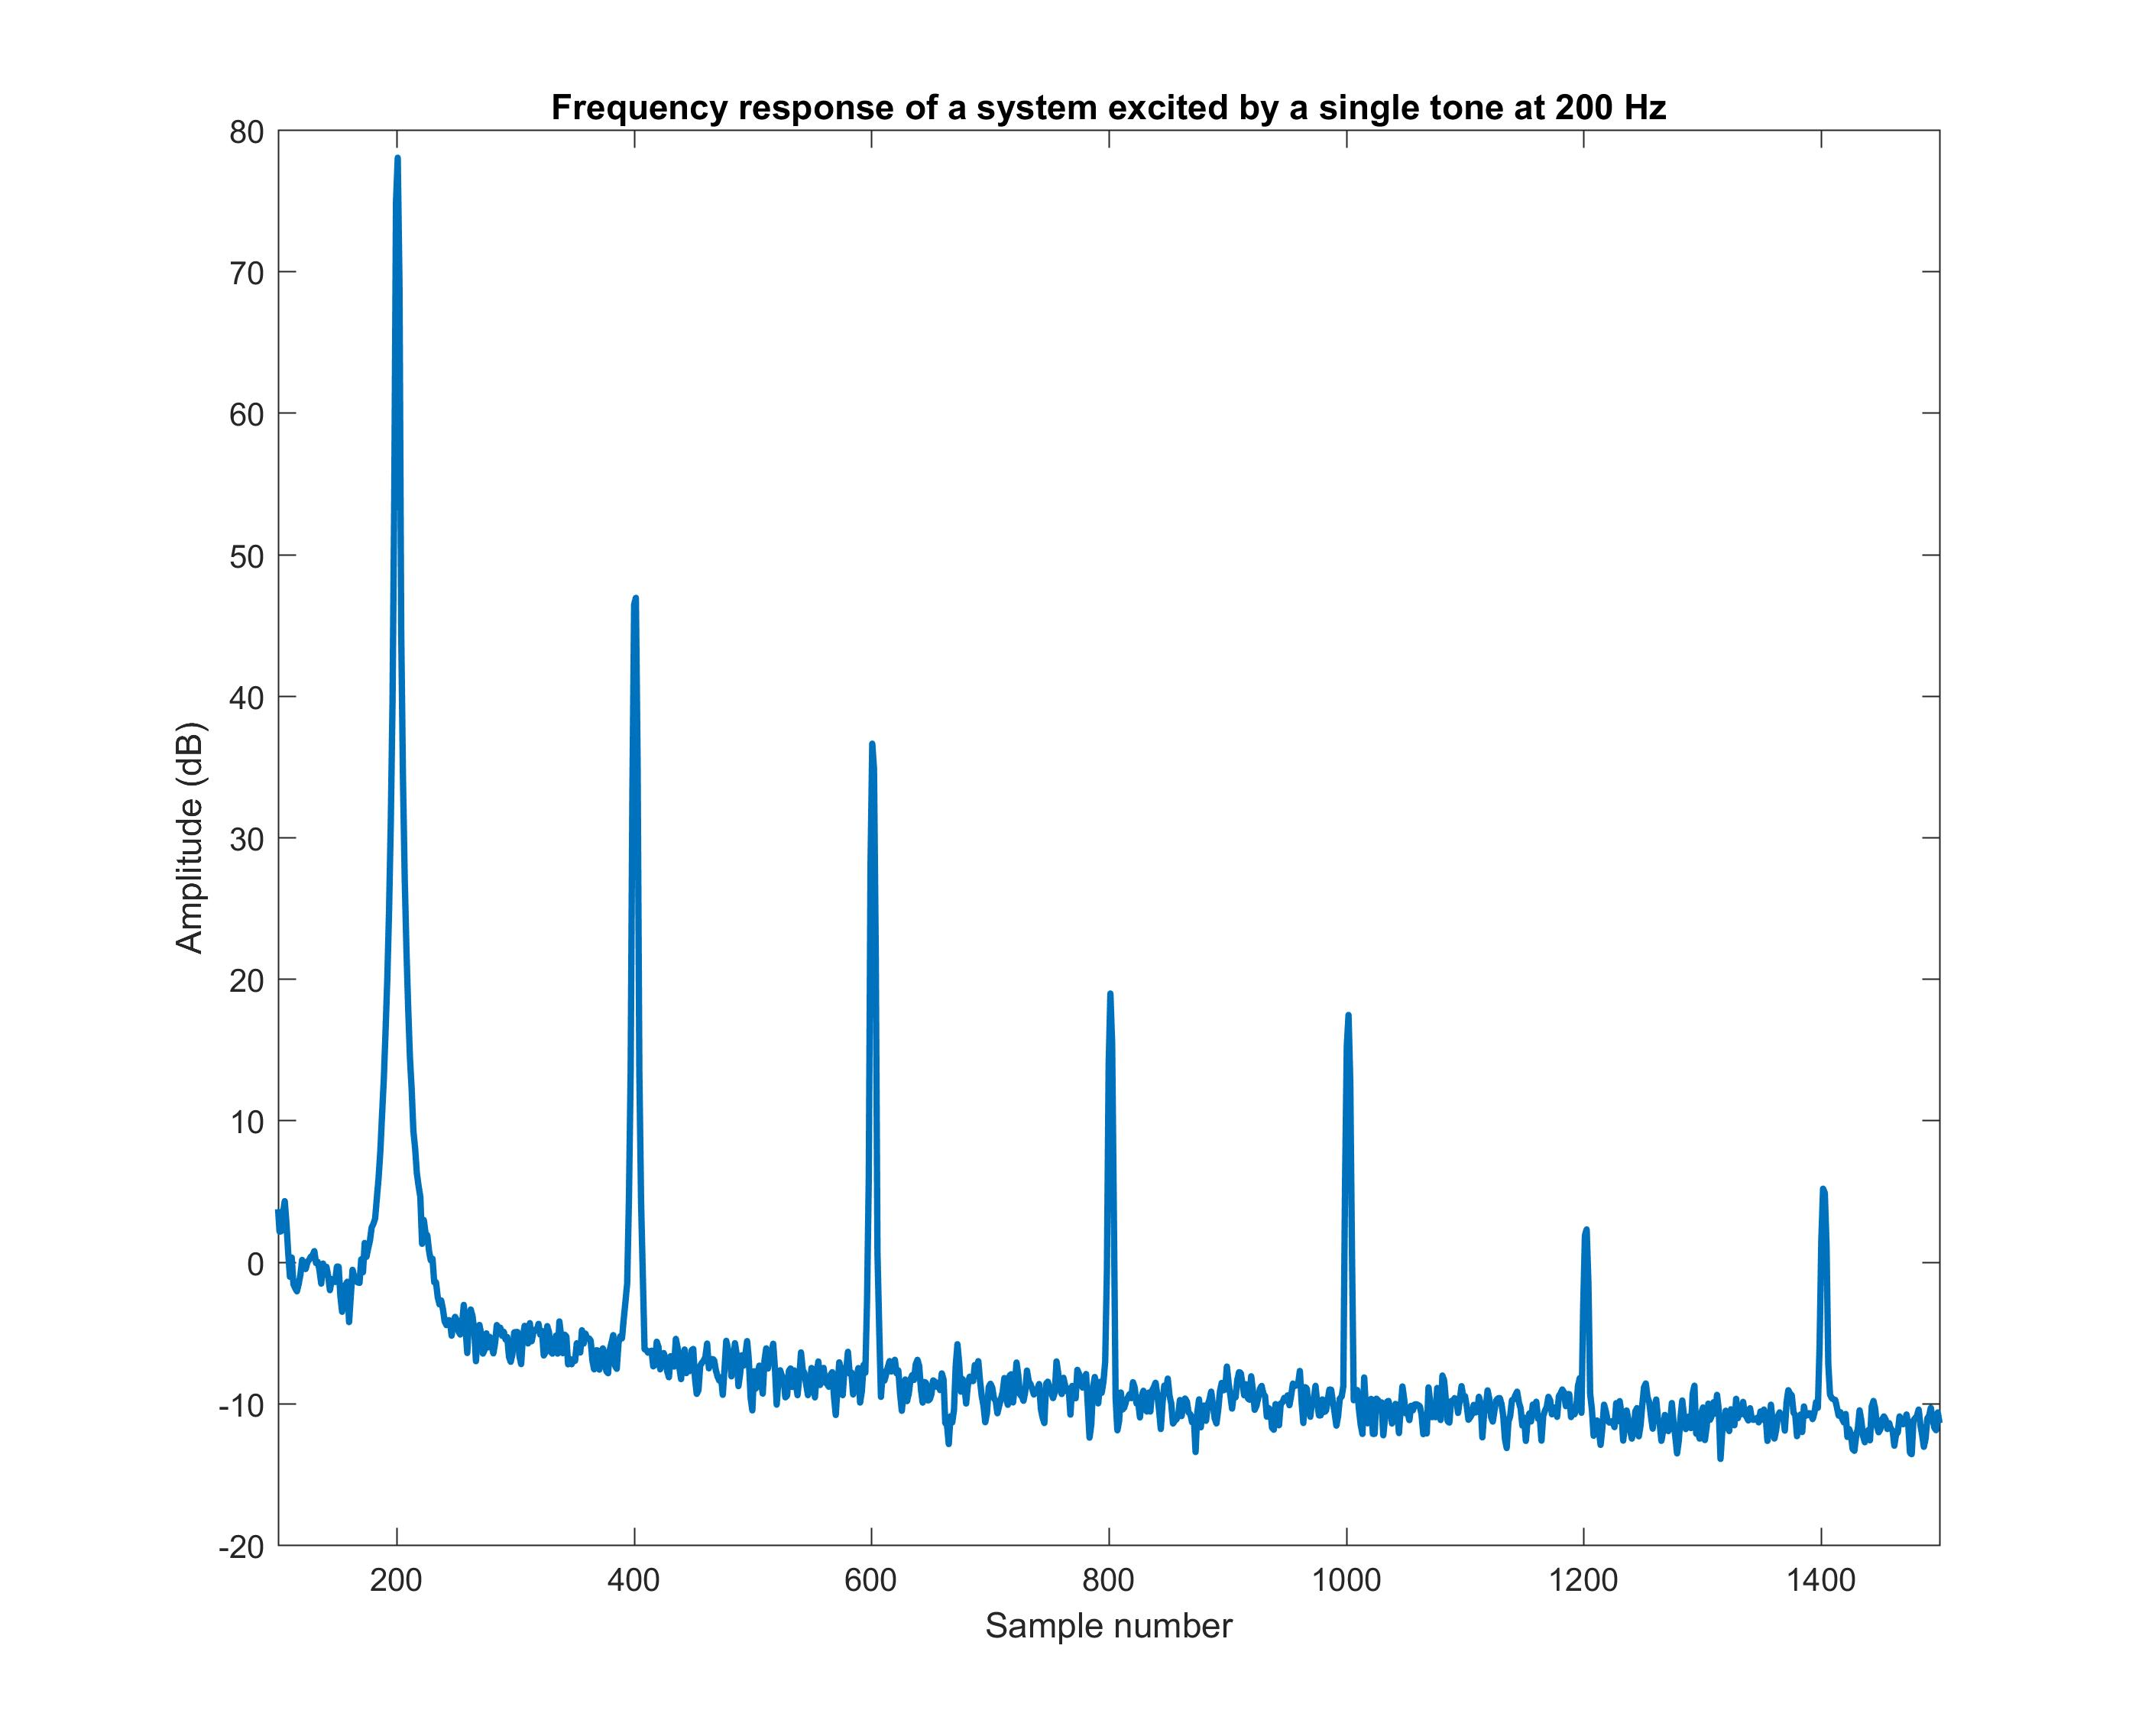
\includegraphics[width=13cm,height=13cm,keepaspectratio]{Figures/frsingletoneanechoic}
\decoRule
\caption[FR single tone]{Frequency response of the system describe in section \ref{subsec:roomsanechoic}, when excited by a $200$Hz sine-wave.}
\label{fig:frsingletone}
\end{figure}
\\
The diagram shows a peak in correspondence of the frequency of tone, plus a series of peaks, the most noticeable ones at integer multiples of the original one. As explained in section ~\ref{sec:soundgen}, this is due to speaker nonlinearities. This kind of measurements have a very high
signal to noise ratio (SNR) because all the energy of the signal is concentrated at one frequency. This, even though can give a good estimation of the (non) linearity of the system, has to be repeated for all the discrete frequencies of interest, which, for high quality sound systems range between [20-20000]Hz, or even more. A Logsweep signal energy spectrum has the convenient property of being able to occupy the whole frequency range specified and, as explained shortly after, can show the system behavior for a continuous range of frequencies.
\\
The Logsweep, also called chirp function, has the interesting property that allows to discern the linear part of the system from its higher order components by separating the impulse responses of the system for each harmonic order.
\\
The function can be mathematically expressed by

\begin{equation}
x(t) = sin \left[ 2 \pi f_1 L e^{\frac{t}{L}} \right];
\label{eqn:logsweep}
\end{equation}

where

\[ L = \frac{1}{f_1} round \left[ \frac{f_1}{ln(\frac{f_2}{f_1})} T \right]; \]
\\
$f_1$ and $f_2$ are the initial and final frequencies, $T$ is the total time of the measurements and $t$ is the instantaneous time with $0<t<T$.
\\
The wave function of a Logsweep is essentially a sine wave whose frequency increases exponentially with time. Multiples of the time of interest, $t$, show a doubling in frequency of the signal. The signal to noise ratio of the calculation is given by the time taken by the sweep, the longer the signal is, the better SNR we get.
\\
The test signal also has ramp-in and ramp-out scaling factors added to it, in order to safeguard the instrumentation. This is achieved by multiplying the first and last couple of thousands samples of the generated chirp tone by a linearly increasing set of values.
\\
A spectrogram of the Logsweep, with duration of 10 seconds, is presented below

\begin{figure}[H]
\centering
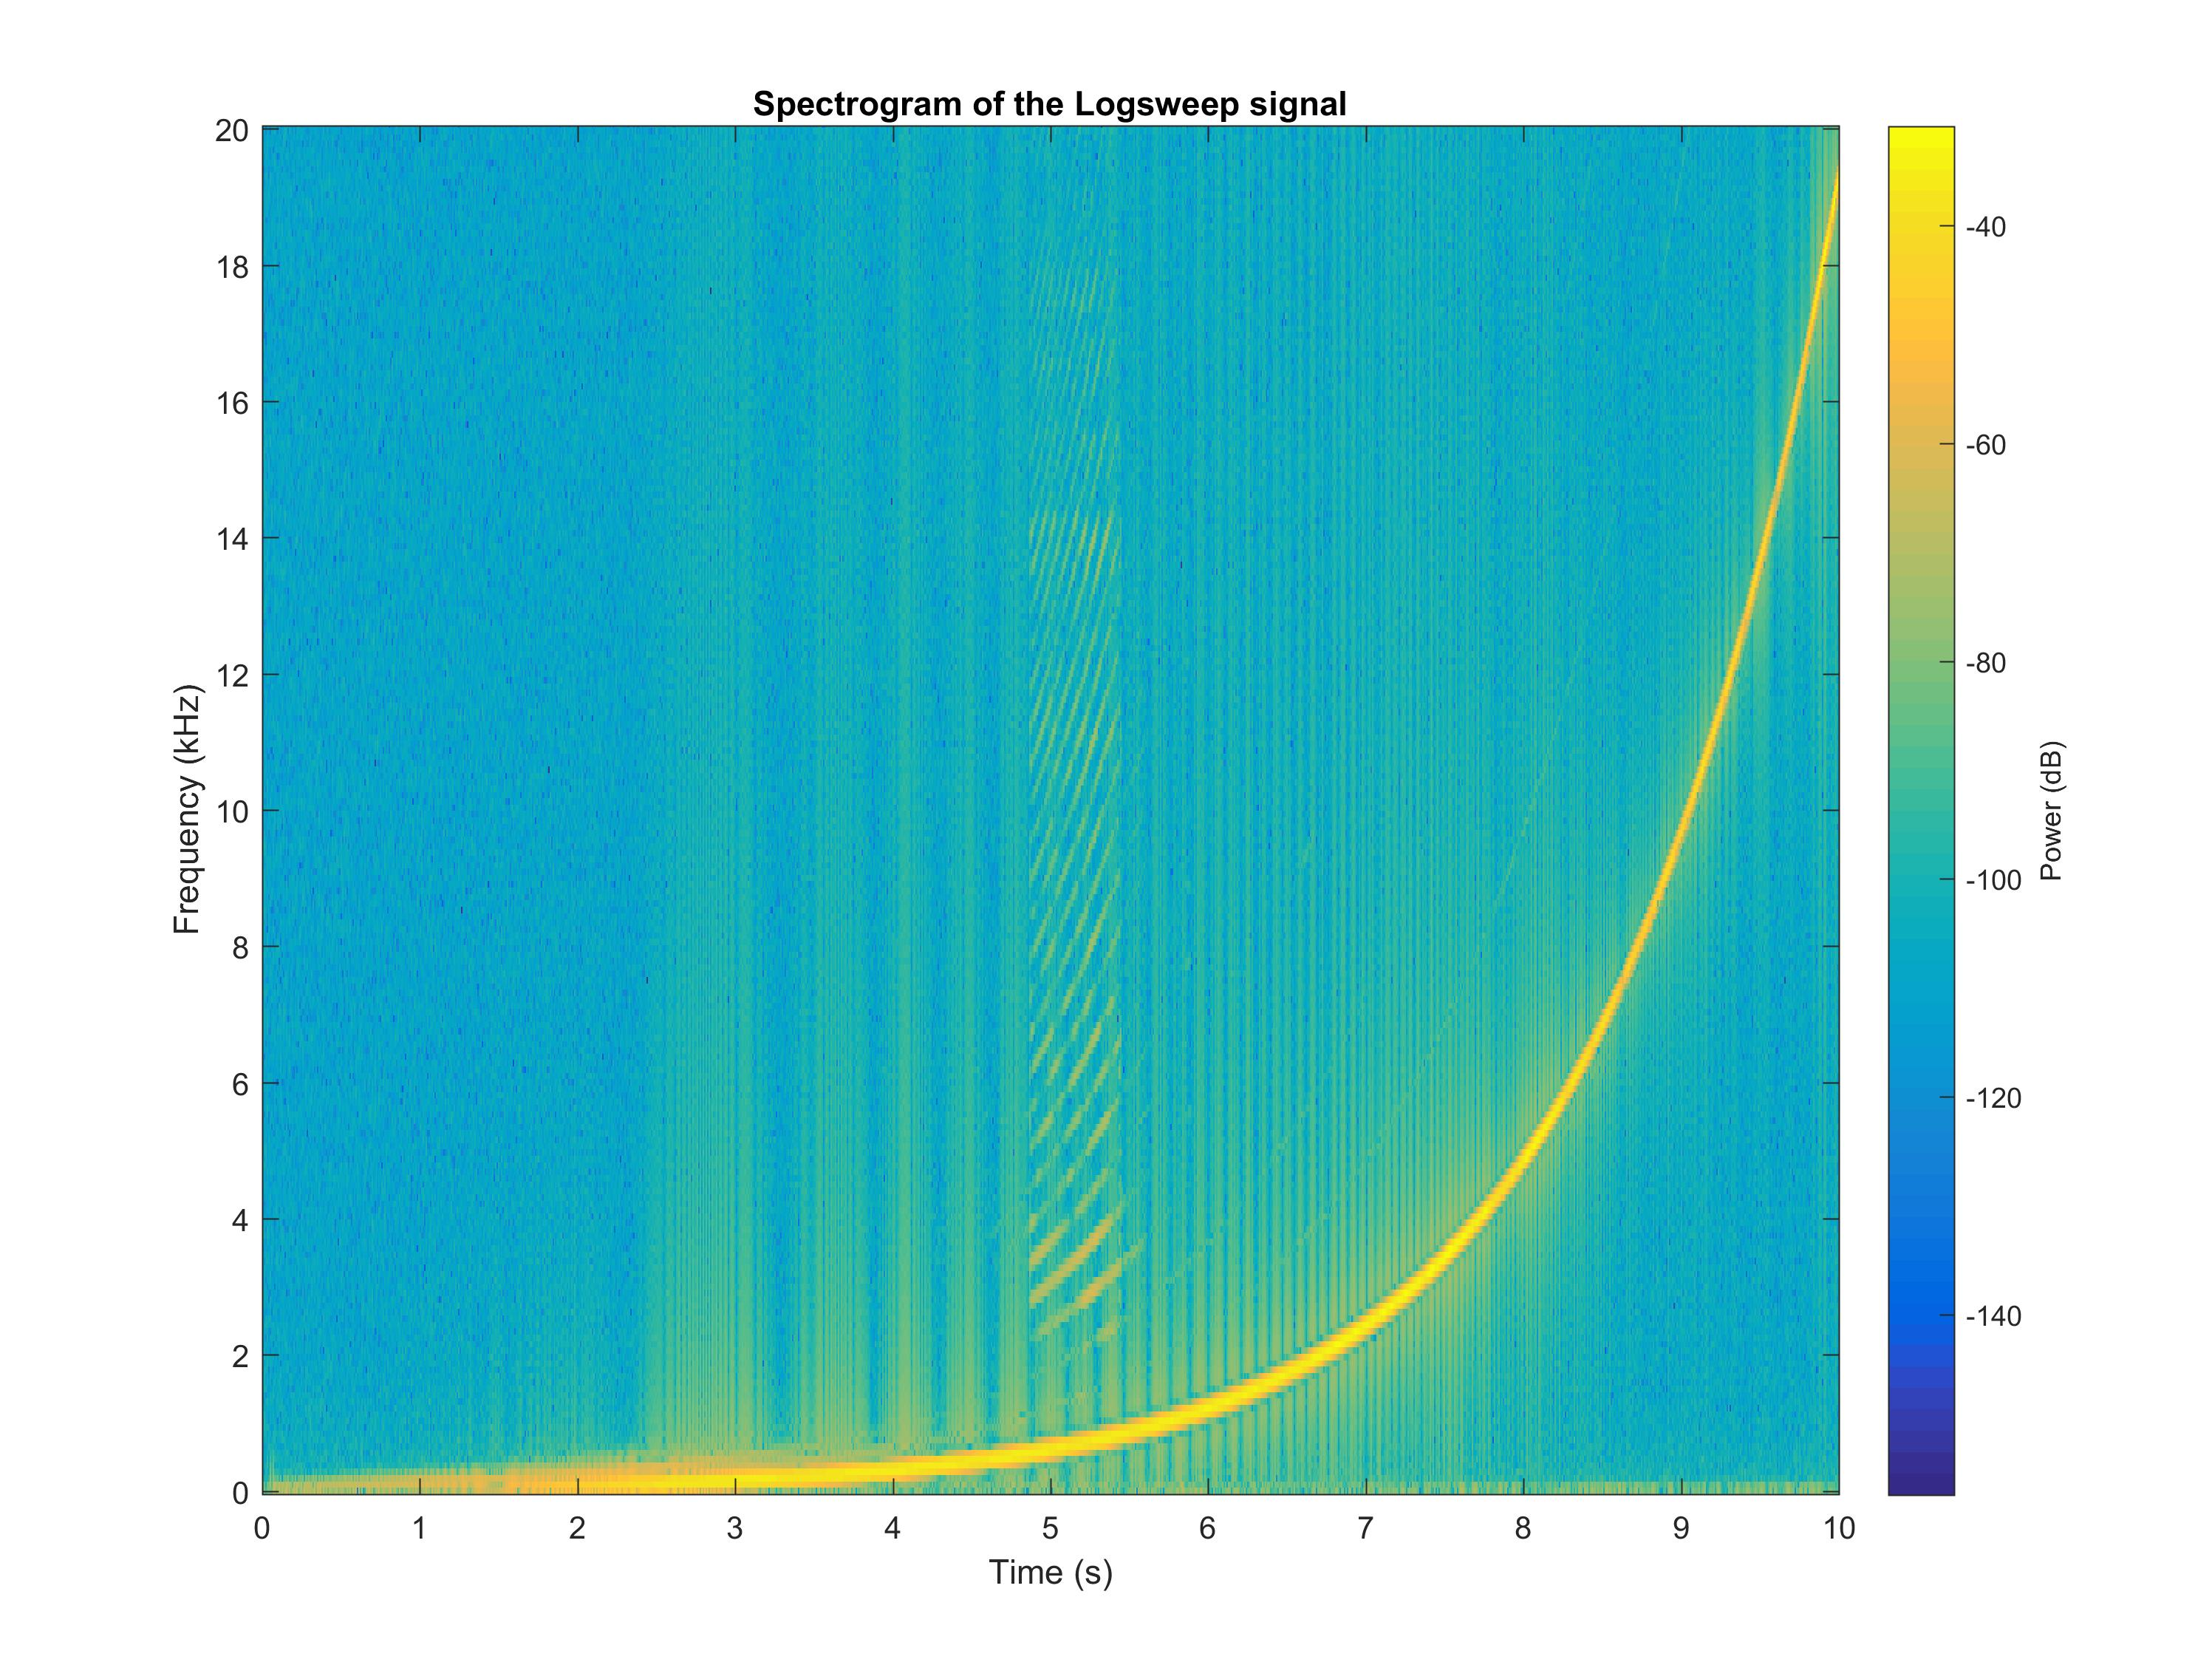
\includegraphics[width=15cm,height=16.5cm,keepaspectratio]{Figures/spectrogramlogsweep}
\decoRule
\caption[Logsweep]{The spectrogram of a Logsweep signal, with ramp-in and ramp-out of 2000 samples. The frequency scale is linear. You can also notice the higher frequencies harmonics when the signal crosses the $200$Hz mark.}
\label{fig:logsweep}
\end{figure}

Once outputted the signal and after having applied equation \ref{eqn:h}, the result is the impulse response of the system, where the harmonic components are well separated. A window filter can be applied to the resulting IR to divide each harmonic order, the frequency band of each one of those is $[nf_1, f_2]$, where $n$ is the number of higher harmonics (HH) we want to study. The graphs representing the fundamental and higher order harmonics of the system used for the tests will be presented in chapter\ref{Chapter4}.
\\
The separation between each HH is equal to $\delta t_n = L ln(n)$, this means, the more HH we want to calculate, the shorter the $\delta t_n$s are.
\\
\\
Finally, we can say that the Fourier transform of $h_n(t)$, $H_n(f)$, represented with a magnitude plot (like the one in figure \ref{fig:frsingletone}) is the most common
representation since it shows the distortion of all the harmonics as a function of the frequency.

\section{Simulated environment}
\label{sec:simenv}

The very first step for reproducing the \parencite{cai_time-domain_2014} BACC-RD algorithm was to design a simulation able to prove the effectiveness of the concept. In order to find a filter able to create some kind of acoustic contrast it was necessary to generate an appropriate impulse response for the simulated environment. The simulation room was composed of 8 ideal sound sources, each one $10$cm apart one another and 32 ideal impulse response detection points, divided in two zones. Each point is $5$cm apart from its neighboring ones. The distance between the simulated sound source and the closest simulated detection point, with respect of the x axis, is $3$m. The simulated room is represented in figure \ref{fig:simroom}.

\begin{figure}[H]
\centering
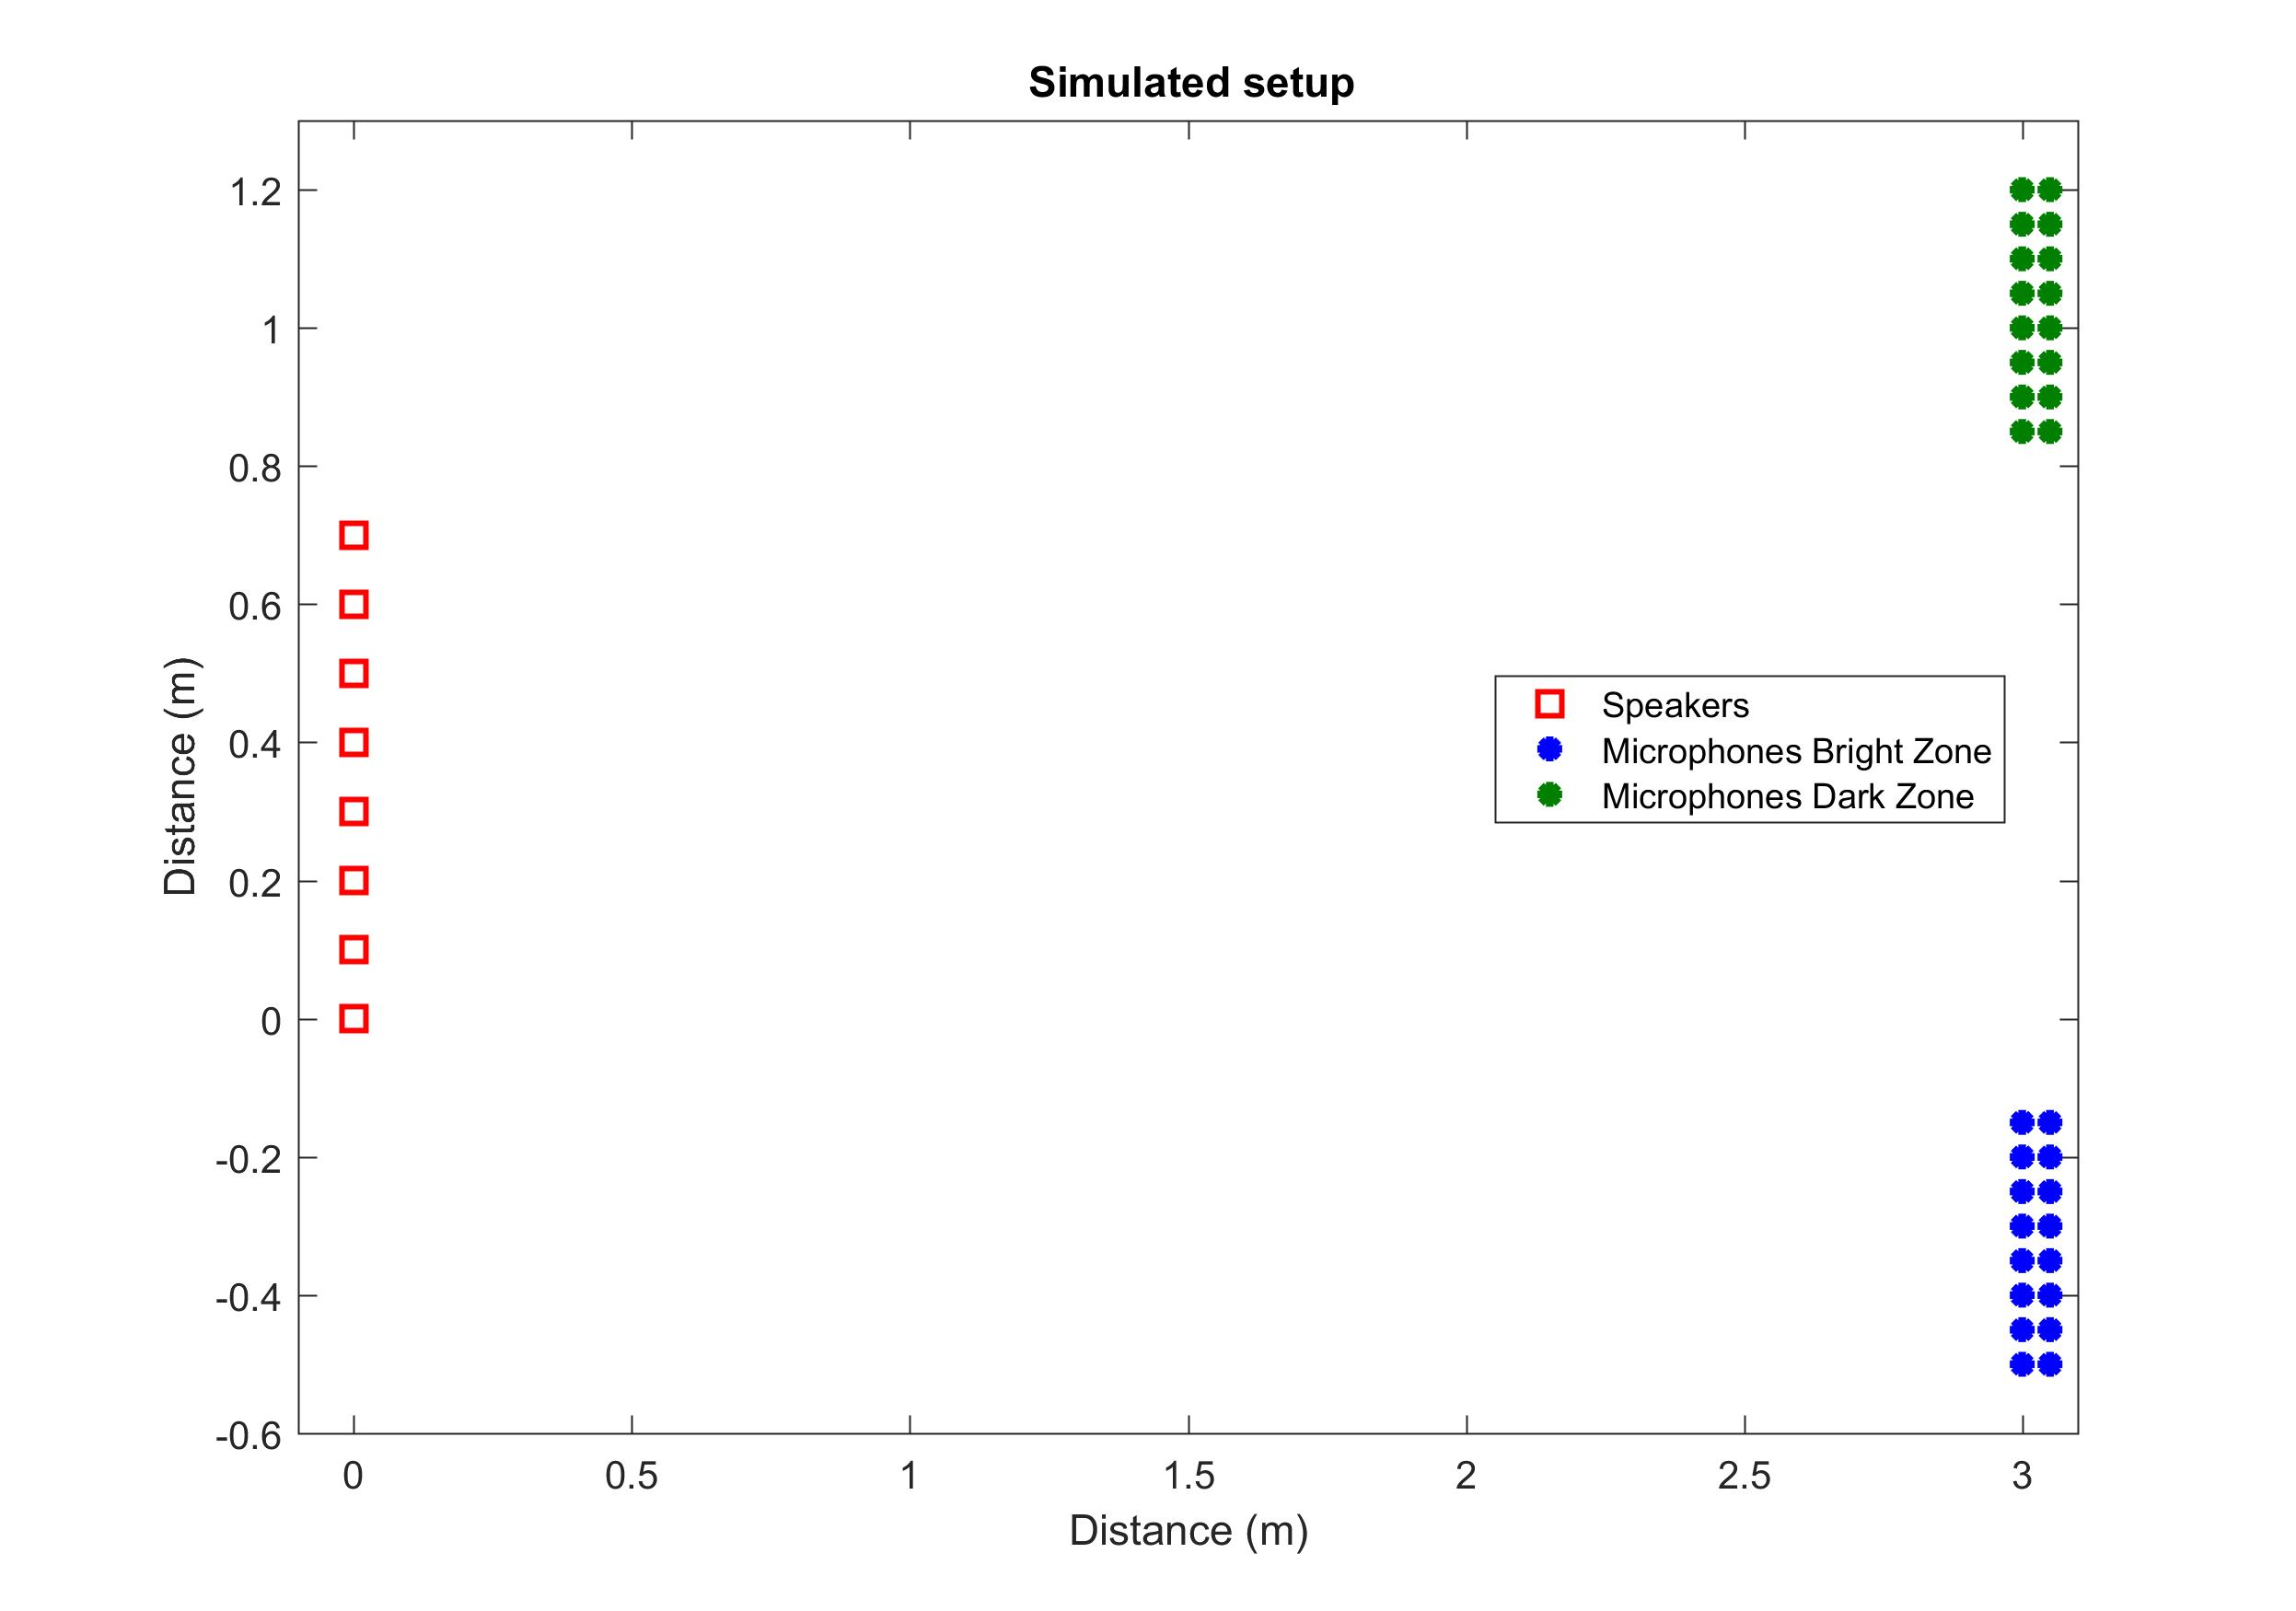
\includegraphics[width=14cm,height=14cm,keepaspectratio]{Figures/simroom}
\decoRule
\caption[Simulated room]{Simulated room. The red stars represent the speaker and the green and blue ones represent the microphones in the two zones.}
\label{fig:simroom}
\end{figure}

As shown in the figure above, the two clusters of detection points are referred to as bright and dark zone, this is because we want to design a filter that is able to limit the total acoustic energy in the area delimited by the green points, while leaving the other zone as unaltered as possible.
\\
Thanks to the Green's function it was possible to design a simulated impulse response of the system. A random signal is supposed to be outputted by each of the red source points (sequentially) and detected by all of the control points in both zones. The propagation of the wave has been calculated using equation \ref{eqn:green}. The intensity and the sample number of the spike that appears on the IR depends on the relative distance between source and detection points and the sampling frequency. This is because the Green's function is expressed also as a function of the distance. The impulse response of the system, as detected in the lower-left point in the bright zone of coordinates (3,-0.5) and emitted by the source of coordinates (0,0) is shown in Figure \ref{fig:simir}. Of course, since the impulse response is in the time domain, the result elaborated by the Green's function has been inverse Fourier Transformed.

\begin{figure}[H]
\centering
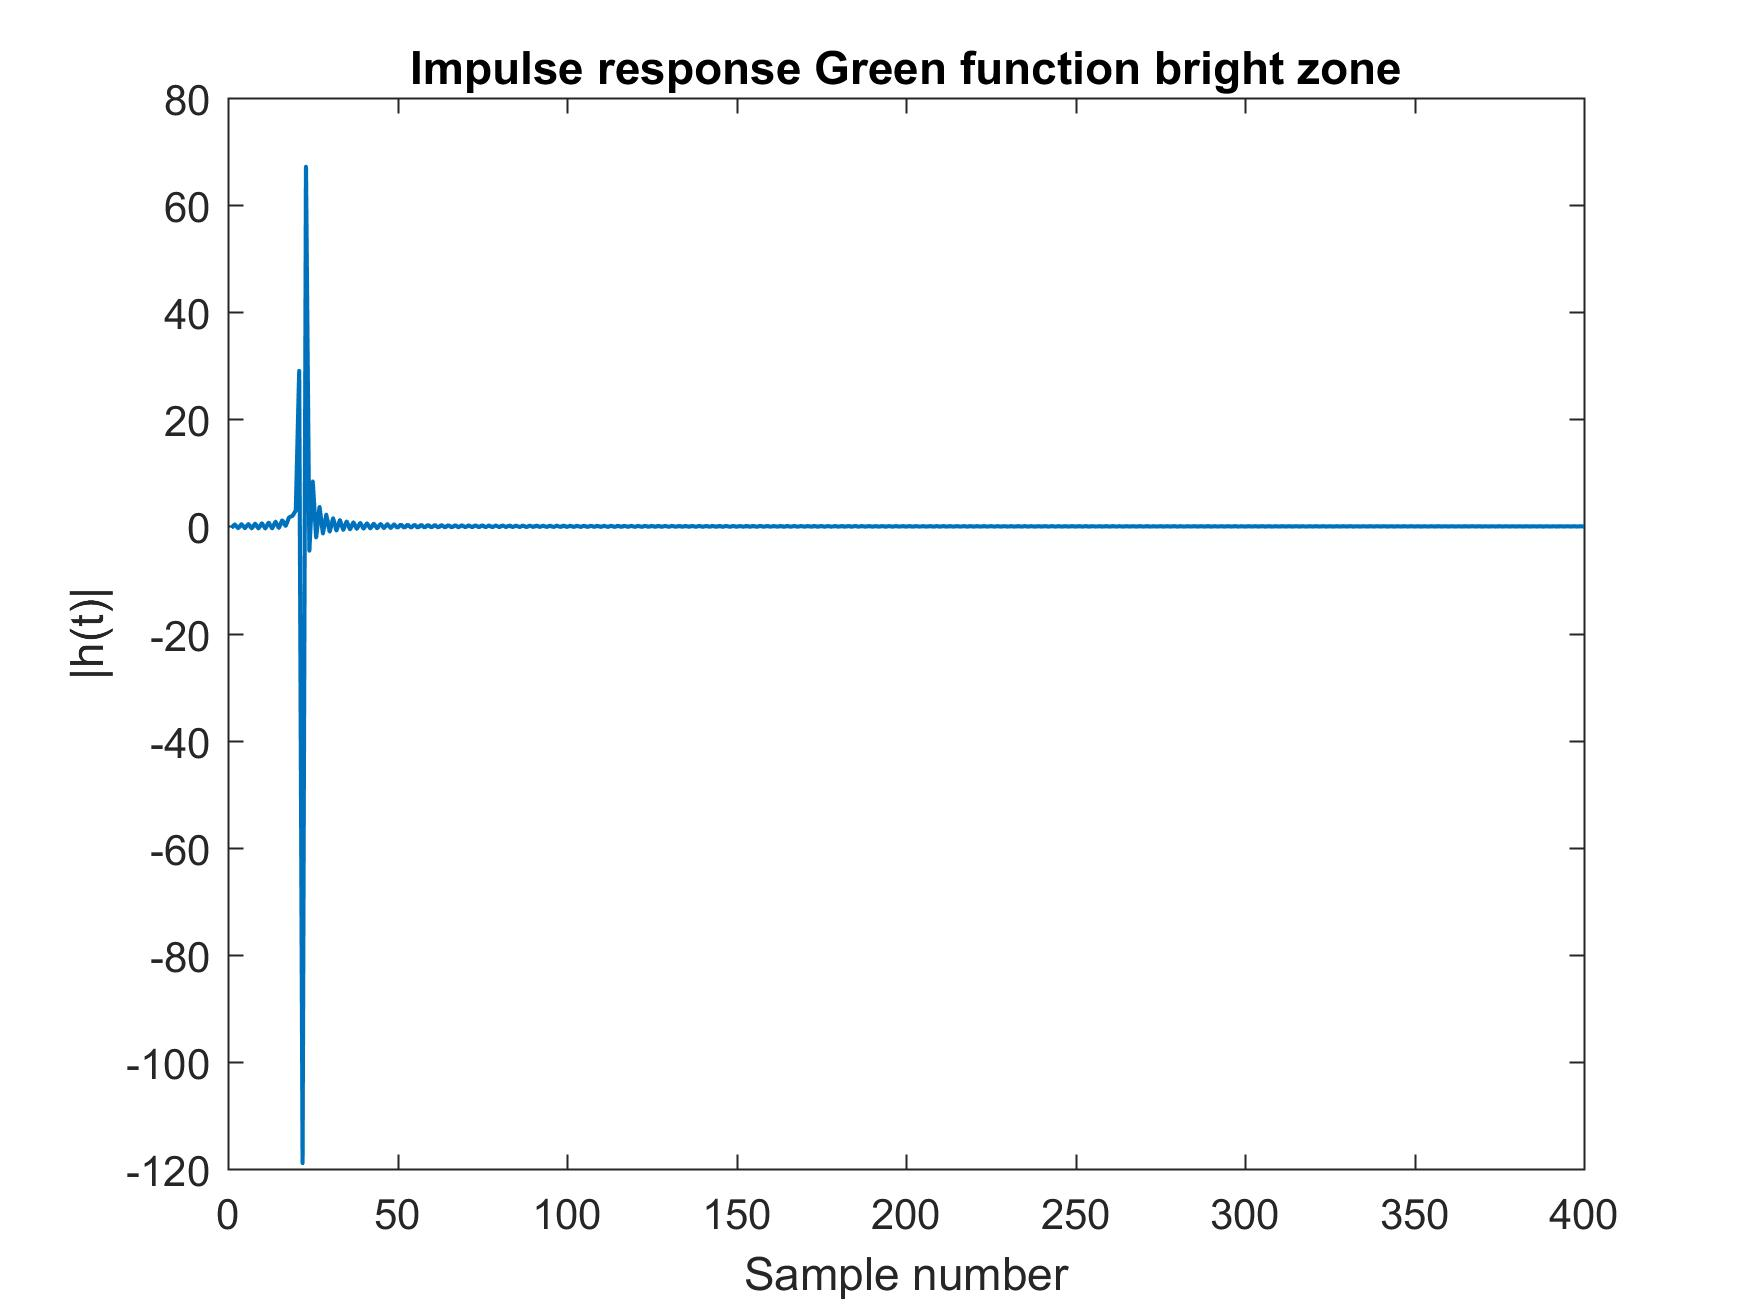
\includegraphics[width=15cm,height=15cm,keepaspectratio]{Figures/simir}
\decoRule
\caption[Simulated IR]{Simulated impulse response of the system using the Green's function.}
\label{fig:simir}
\end{figure}

If we were to replicate the same configuration in figure \ref{fig:simroom} of speakers and sound zones in any real environment, even the anechoic chamber, and apply the BACC-RD algorithm to generate some acoustic contrast, we would have had a lower result with respected of the one obtained in the simulation. This is ascribable to the fact that the power amplifiers and A/D converters add noise (either in the analog or digital domain, noise can be expressed in terms of bit error rate in the latter), the inherent noise in the microphones and the reflections present in the room, which, of course, cannot be \textit{completely} anechoic, especially when dealing with wideband signals, the kind used in all the ACC scenarios evaluated.
\\
This parting from the simulation shouldn't surprise the reader, since it is the price one has to pay when having to deal with real equipment. Still, the simulated environment has to be considered a development tool for the algorithm itself, we will prove that we are able to achieve acoustic contrast using the hardware described later in this chapter.
\\
\section{The test rooms}
\label{sec:rooms}

The simulated environment, generated using MATLAB, proved fundamental for debugging and checking the validity of the code implementing the BACC-RD algorithm. But, for the reasons already explained in \ref{sec:soundgen}, a simulation using the Green's function is insufficient to analyze the performance of the algorithm in a real environment. In the section below the reader will find a description of the rooms used for running the tests.

\subsection{Anechoic chamber}{}
\label{subsec:roomsanechoic}

The room used for most of the tests was the anechoic chamber in the AUDIOLAB facilites of the Aarhus University. The reader should assume that all the test were conducted in the chamber, unless otherwise specified. The chamber is a test room rated for sound experiments. Both the floor, the walls and the ceiling are acoustically dampened by acoustic foam. The foam in most of the surfaces has a length of $85$cm This means that its effectiveness in dampening the sound is limited to waves roughly shorter than $\frac{1}{4} \lambda = 3.40$m, or \tld$100$Hz.

\begin{figure}[H]
\centering
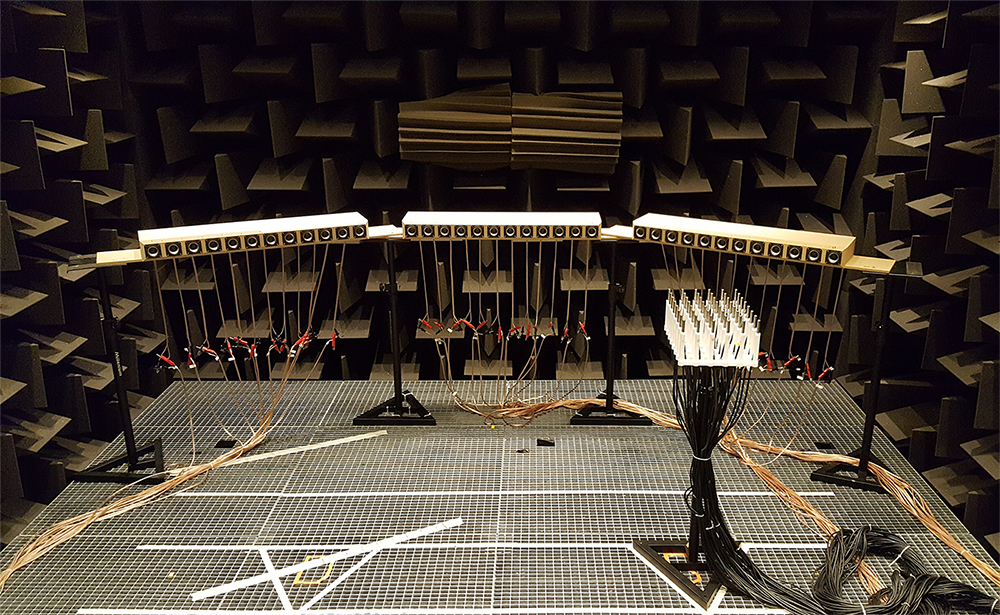
\includegraphics[width=14cm,height=15cm,keepaspectratio]{Figures/anechoic}
\decoRule
\caption[Anechoic chamber]{The anechoic chamber in the AUDIOLAB facility of the Aarhus University.}
\label{fig:anechoic}
\end{figure}

The chamber dimensions are $6\text{x}5\text{x}4.5$m (length, width, height). The walkable area is made by a metal grid, standing $1.20$m above the actual floor level. The grid is mechanically dampened from the rest of the room. The equipment is secured on the pavement with plastic straps in order to reduce vibrations.
\\
The background noise of the room is \tld$17$dB, this was measured by making a $10$ seconds recording of the room (without playing any sound).

\subsection{Listening room}{}

The second test environment was the listening room of the AUDIOLAB facility in the Aarhus University. It is a room designed to simulate a real living room environment, with chairs, tables and bookshelves. The furniture provides a multitude of reflective surfaces that spread the sound, meaning that the reverberation time is understandably higher than the one in the anechoic chamber. This room has been used to demonstrate the feasibility of the study in an every day scenario.
The room dimensions are $4.75\text{x}4.75\text{x}2.70$m (length, width, height).

\begin{figure}[H]
\centering
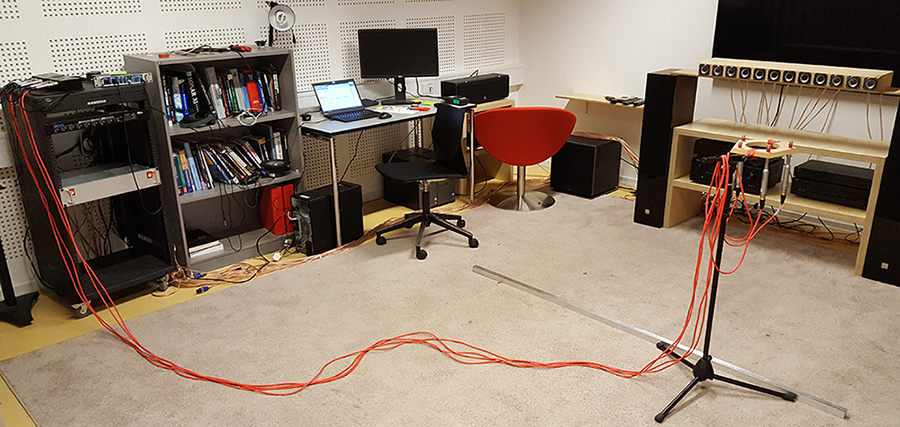
\includegraphics[width=14.5cm,height=15cm,keepaspectratio]{Figures/listeningv2}
\decoRule
\caption[Listening chamber]{The listening room of the AUDIOLAB facility.}
\label{fig:listening}
\end{figure}

The background noise in this room is \tld$25$dB. This value is measured when the instruments (especially the power amplifiers, which have active cooling) inside the room were turned on.

\section{Hardware}
\label{sec:hw}

This sections provides some details regarding the hardware that allows the change of domain of the signal, specifically from the digital domain of the data coming from the PC running MATLAB to the analog domain used by the loudspeaker, to the mechanical domain of the sound recorded by the microphones, only to be converted back to an analog and then digital signal returned to the PC.

\subsection{A/D converters}{}

The conversion from and to the PC running the MATLAB code was performed by some A/D and D/A converters. The ones used for the anechoic chamber are respectively an RME M-32 AD and an RME M-32 DA. Each one of them is equipped with 32-channels. Since the total numbers of speakers in the chamber is $36$ and the microphones in the matrix are $48$, two unit of each converter are used. These pieces of hardware are daisy chained through an optical connection that provides an useful single interface to communicate with the PC. Thanks to Playrec it was enough to specify the target device (a digital interface) and the firmware of the converters themselves took care of synchronization and delivery of the signals between the units.
\\
the D/A converters are connected to two ICEpower1000ASP power amplifiers. These unit are the ones directly connected to the loudspeakers in the anechoic chamber. A gain attenuator of $-20$dB is used in each line after the amplification, to prevent damage to the loudspeakers.
\\
The A/D converter are connected to the custom microphone power amplifiers (inside the chamber) that power up the Panasonic microphones (the ones in figure \ref{fig:anechoic}).
An additional line of the A/D is reserved for an Nti microphone (described in section \ref{subsec:mics}), which requires its own phantom power, positioned in the signal chain between the two, specifically, the power unit used is a Millennium PP2B.
\\
One data line is directly connected from the D/A to the A/D converter. This lines bypasses the loudspeakers and microphones completely. Feeding data trough this channel reveals how long of a delay having this equipment introduces into the signal chain. It is also a useful monitor that allows us to see if the input signal, intended to the loudspeakers is correct.
\\
\\
The listening room is provided with some more portable hardware, namely the RME Fireface UC, which acts as A/D and D/A converter. The Fireface output lines are connected to a single ICEpower amplifier, which drives the loudspeakers. A gain attenuator of $-20$dB is used again. The microphones are powered by two other Millennium PP2B units, which have 2 I/O lines each, similarly as the one used in the anechoic chamber.

All the converters allow for two different sampling frequencies, $48$kHz or $96$kHz, the one that will always used will be the former.

\subsection{Loudspeakers}{}
\label{subsec:speakers}

The choice of the best set of loudspeakers among the available ones has been the first development steps of this project. Checking the inventory of the laboratory, two were the models deemed suitable. The SB acoustics SB65WBAC25-4 $2.5$ inches and the AuraSound NS2-326-8AT $2$ inches speakers.
\\
The first one has an impedance of $4$Ohm and a power capacity of $20$W RMS. The second has an higher impedance of $8$Ohm, but can output a maximum of $15$W RMS.

\begin{figure}[H]
\centering
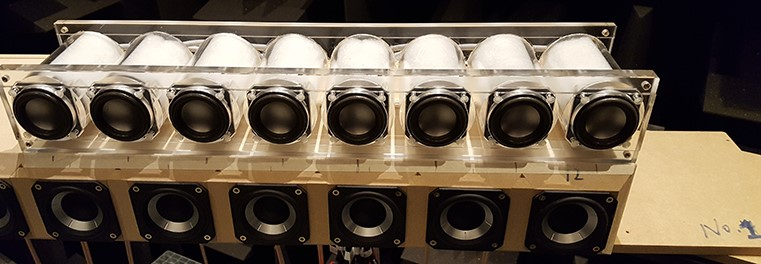
\includegraphics[width=10cm,height=10cm,keepaspectratio]{Figures/aurasb1}
\decoRule
\caption[Aura speakers]{Aura speakers array on top of the SB array on the left side of the anechoic chamber.}
\label{fig:aurasbspeakers}
\end{figure}

The frequency response of the two models is presented below. The speaker used for this measurement are the ones in the figure above, all 8 speakers of the Aura unit (on top) and the 6 rightmost speakers of the first for the SB array (the array on the left in figure \ref{fig:anechoic}). The SPL level has been measured five times and the results averaged, using the same identical input signal (a Logsweep signal lasting for 10 seconds), the results show an SPL of $98.0$dB $\pm0.2$dB for the Aura and $97.1$dB $\pm0.3$dB for the SB arrays. The microphone used was the Nti model at a distance of $1$m.

\begin{figure}[H]
\centering
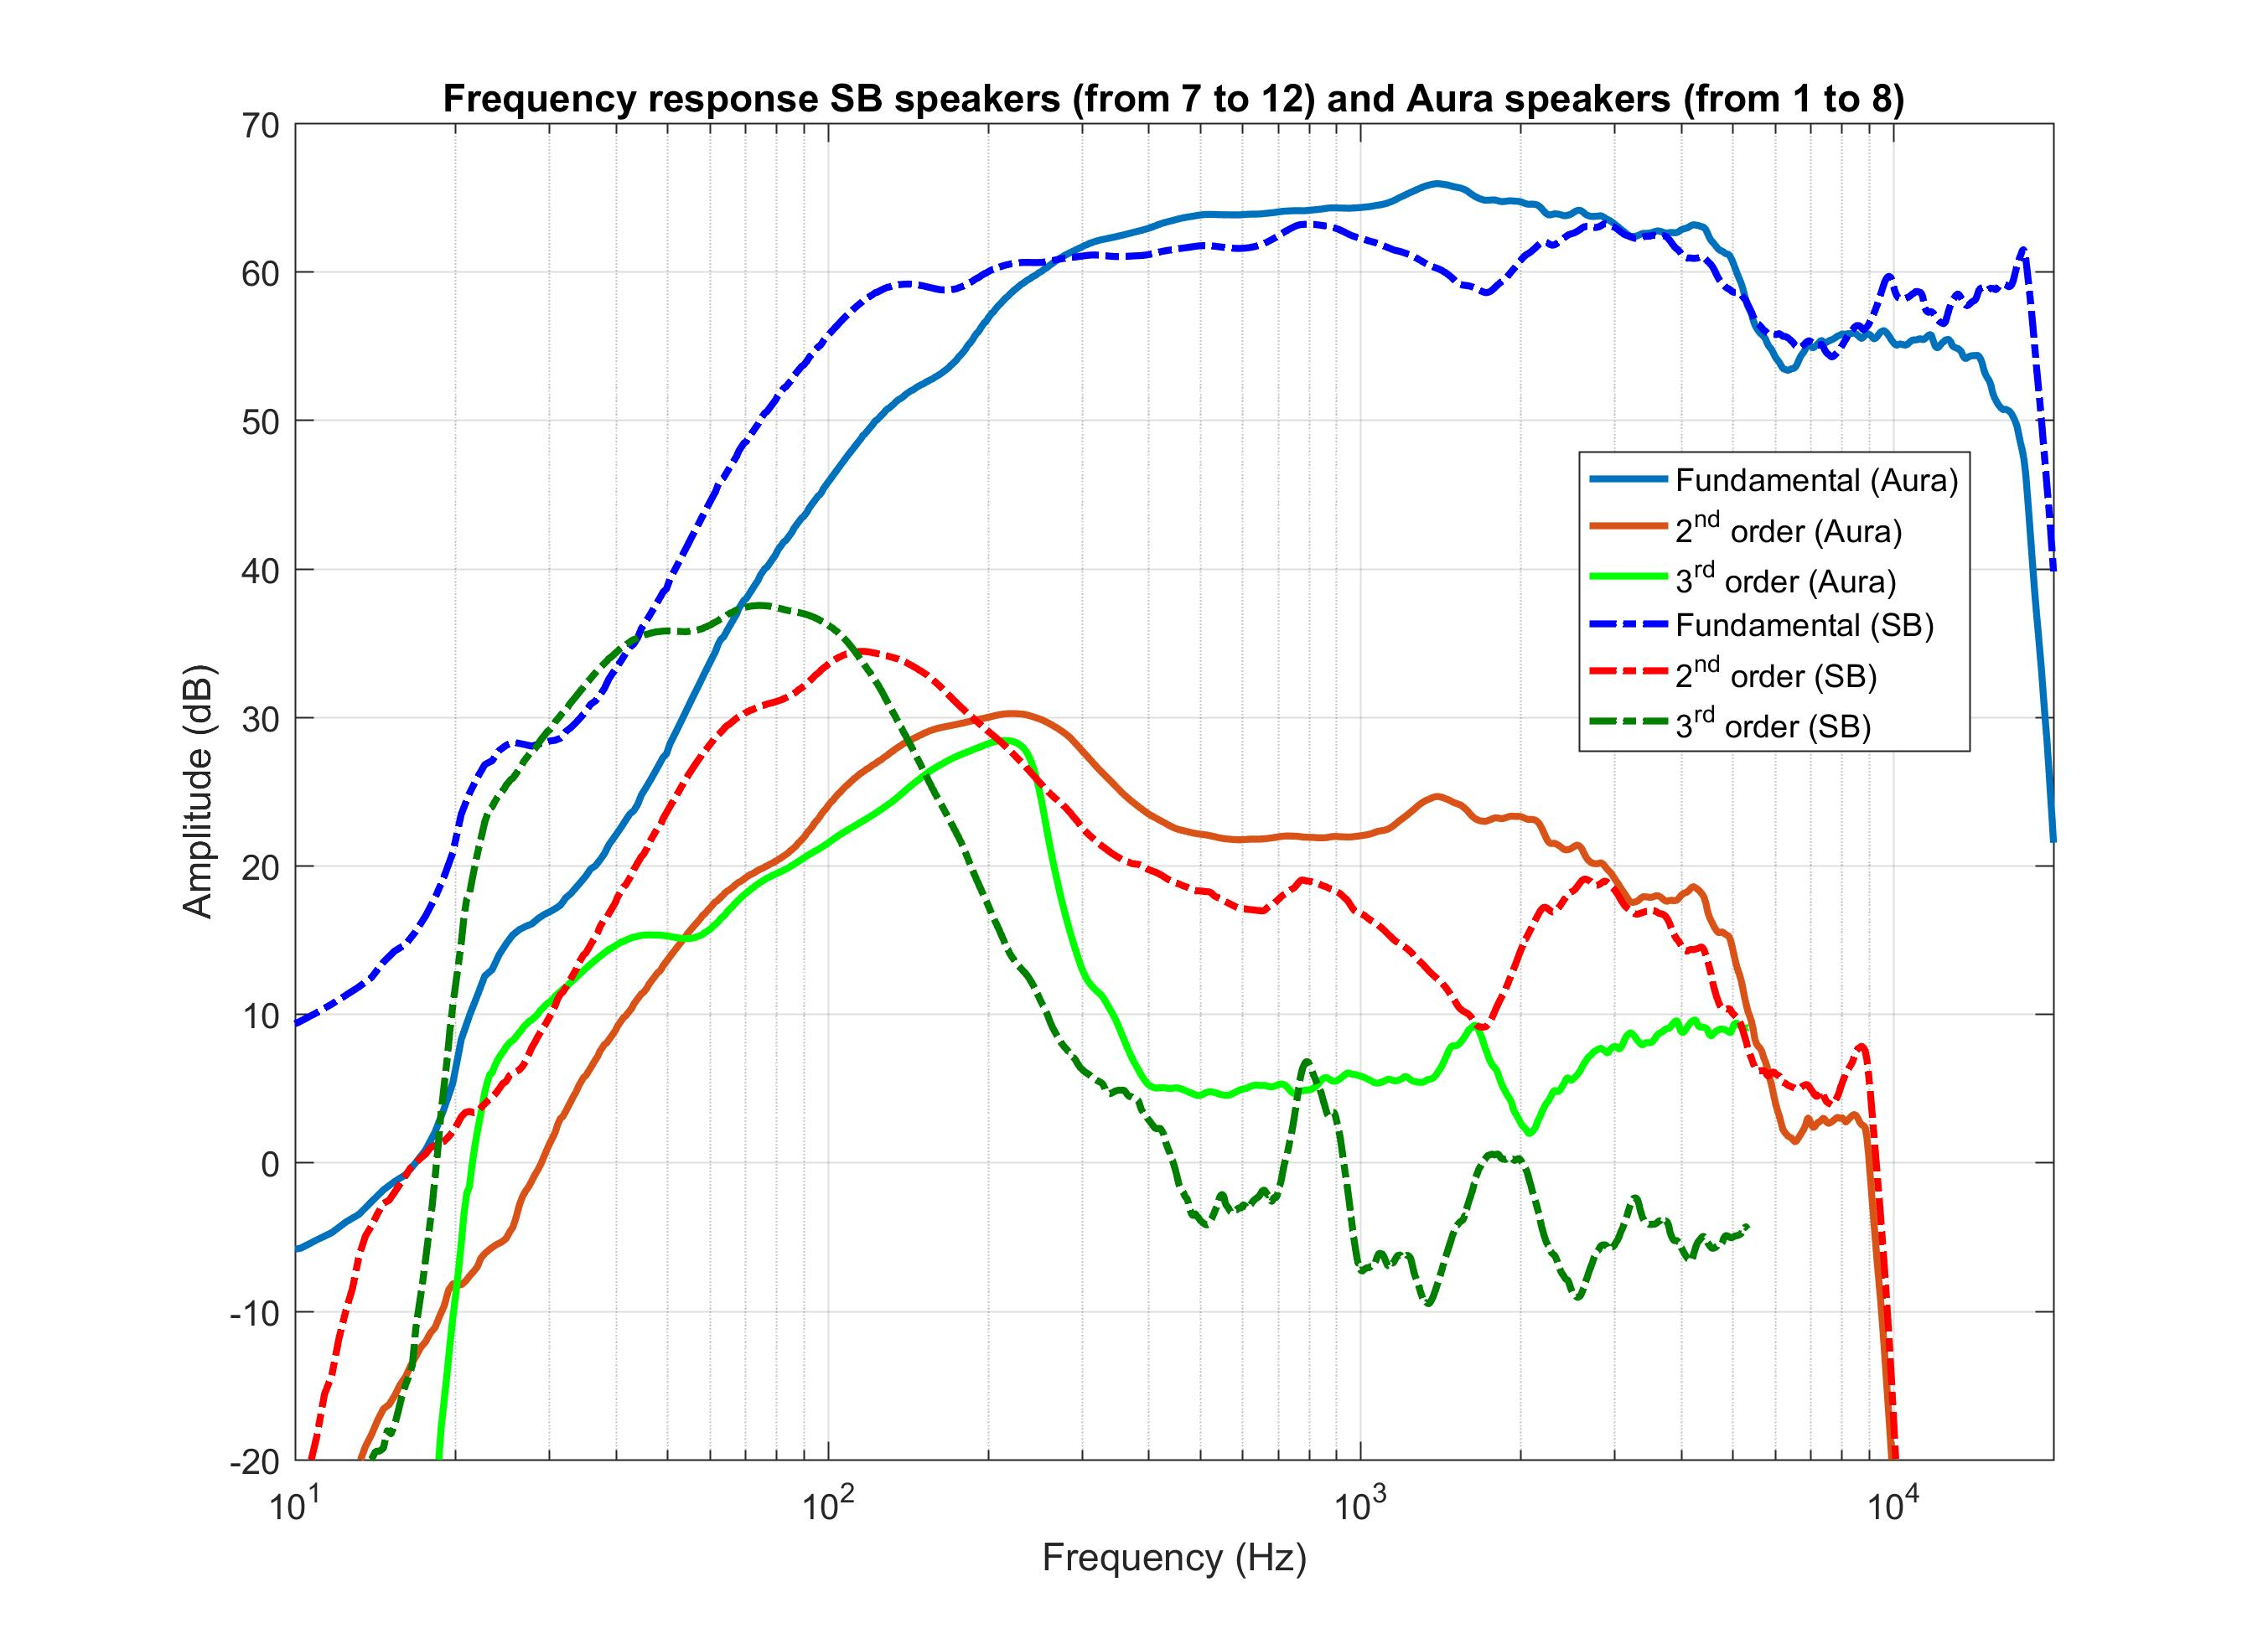
\includegraphics[width=15cm,height=15cm,keepaspectratio]{Figures/aurasbfreq}
\decoRule
\caption[Anechoic chamber]{Comparison between the frequency response of the SB speakers (dotted line) and Aura speakers (solid line). The first 3 harmonics are represented here.}
\label{fig:aurasbfreq}
\end{figure}

In section \ref{sec:soundgen} we explained how the amplitude is an important parameter when it comes to determine the amount of distortion generated by speakers playing a sound. Since the two models have different characteristics, we need to make sure to use a sound level that is comparable. This is done by scaling the amplitude of the input signal $-1\le x\le 1$ using the formula
\[x=\text{input signal}^{(\text{output level in relative scale}/20)}\]

This means that we are going to use a relative scale, which is a pure number, to represent the output level. The maximum value allowed in this scale is $0$, any value beyond this point will be translated by the amplifiers in a value that will end up damaging the speakers.
\\
We can then convert this relative scale to a value in decibels by dividing the root mean square value of the recorded Logsweep signal to the reference sound pressure level (SPL), which is $2\textbf{x}10^{-5}$Pa. Expressed in mathematical notation it can be written as
\[\text{SPL in dB}= 20 \log_{10} \left[\text{rms}(x)/ \text{reference SPL} \right]\]
\\
In the following table we present the conversion between the SPL and the relative scale for the loudspeakers belonging to the central array of SB units, the driver playing were from 15 to 22. The reason why this results presented are for those specific driver units is because, as we will later explain, those were the exact units chosen to carry out most of the experiments of chapter \ref{Chapter4}, hence the following table will be an useful tool to convert the relative scale to a dB value. The conversion only has meaning in the anechoic conditions, changing environment (using, for instance, the listening room) or position of the microphones means we have to re-calculate the correspondence between relative scale and the corresponding SPL, the usefulness of this conversion is given by the fact that the many experiments in the anechoic chamber will almost never see the position of the microphones change (except in those rare case when it will be specified). The recorded SPL level is made by averaging the recordings of the Panasonic microphones (described in the next section) $20, 21, 28, 29$ (the four innermost in the microphone matrix in figure \ref{fig:mics}) situated in the bright zone, $1.40$m from the center of the speakers. This experiment was repeated five times. The margin of error of the measurement was $\pm 0.3$dB.

\begin{table}[H]
\label{tab:relativescale}
\centering
\begin{tabular}{ll}
\toprule
Relative scale & SPL (dB)\\
\midrule
-40            & 69.60\\
-35            & 74.60\\
-30            & 79.70\\
-25            & 84.50\\
-20            & 89.50\\
-15            & 94.10\\
-10            & 98.20\\
\bottomrule\\
\end{tabular}
\caption{Comparison between output level and corresponding SPL.}
\label{tab:relativescale}
\end{table}

If we graph the two scales together we can see that the amplification is pretty much linear, which is to be expected when applying different gains to the input signal.

\begin{figure}[H]
\centering
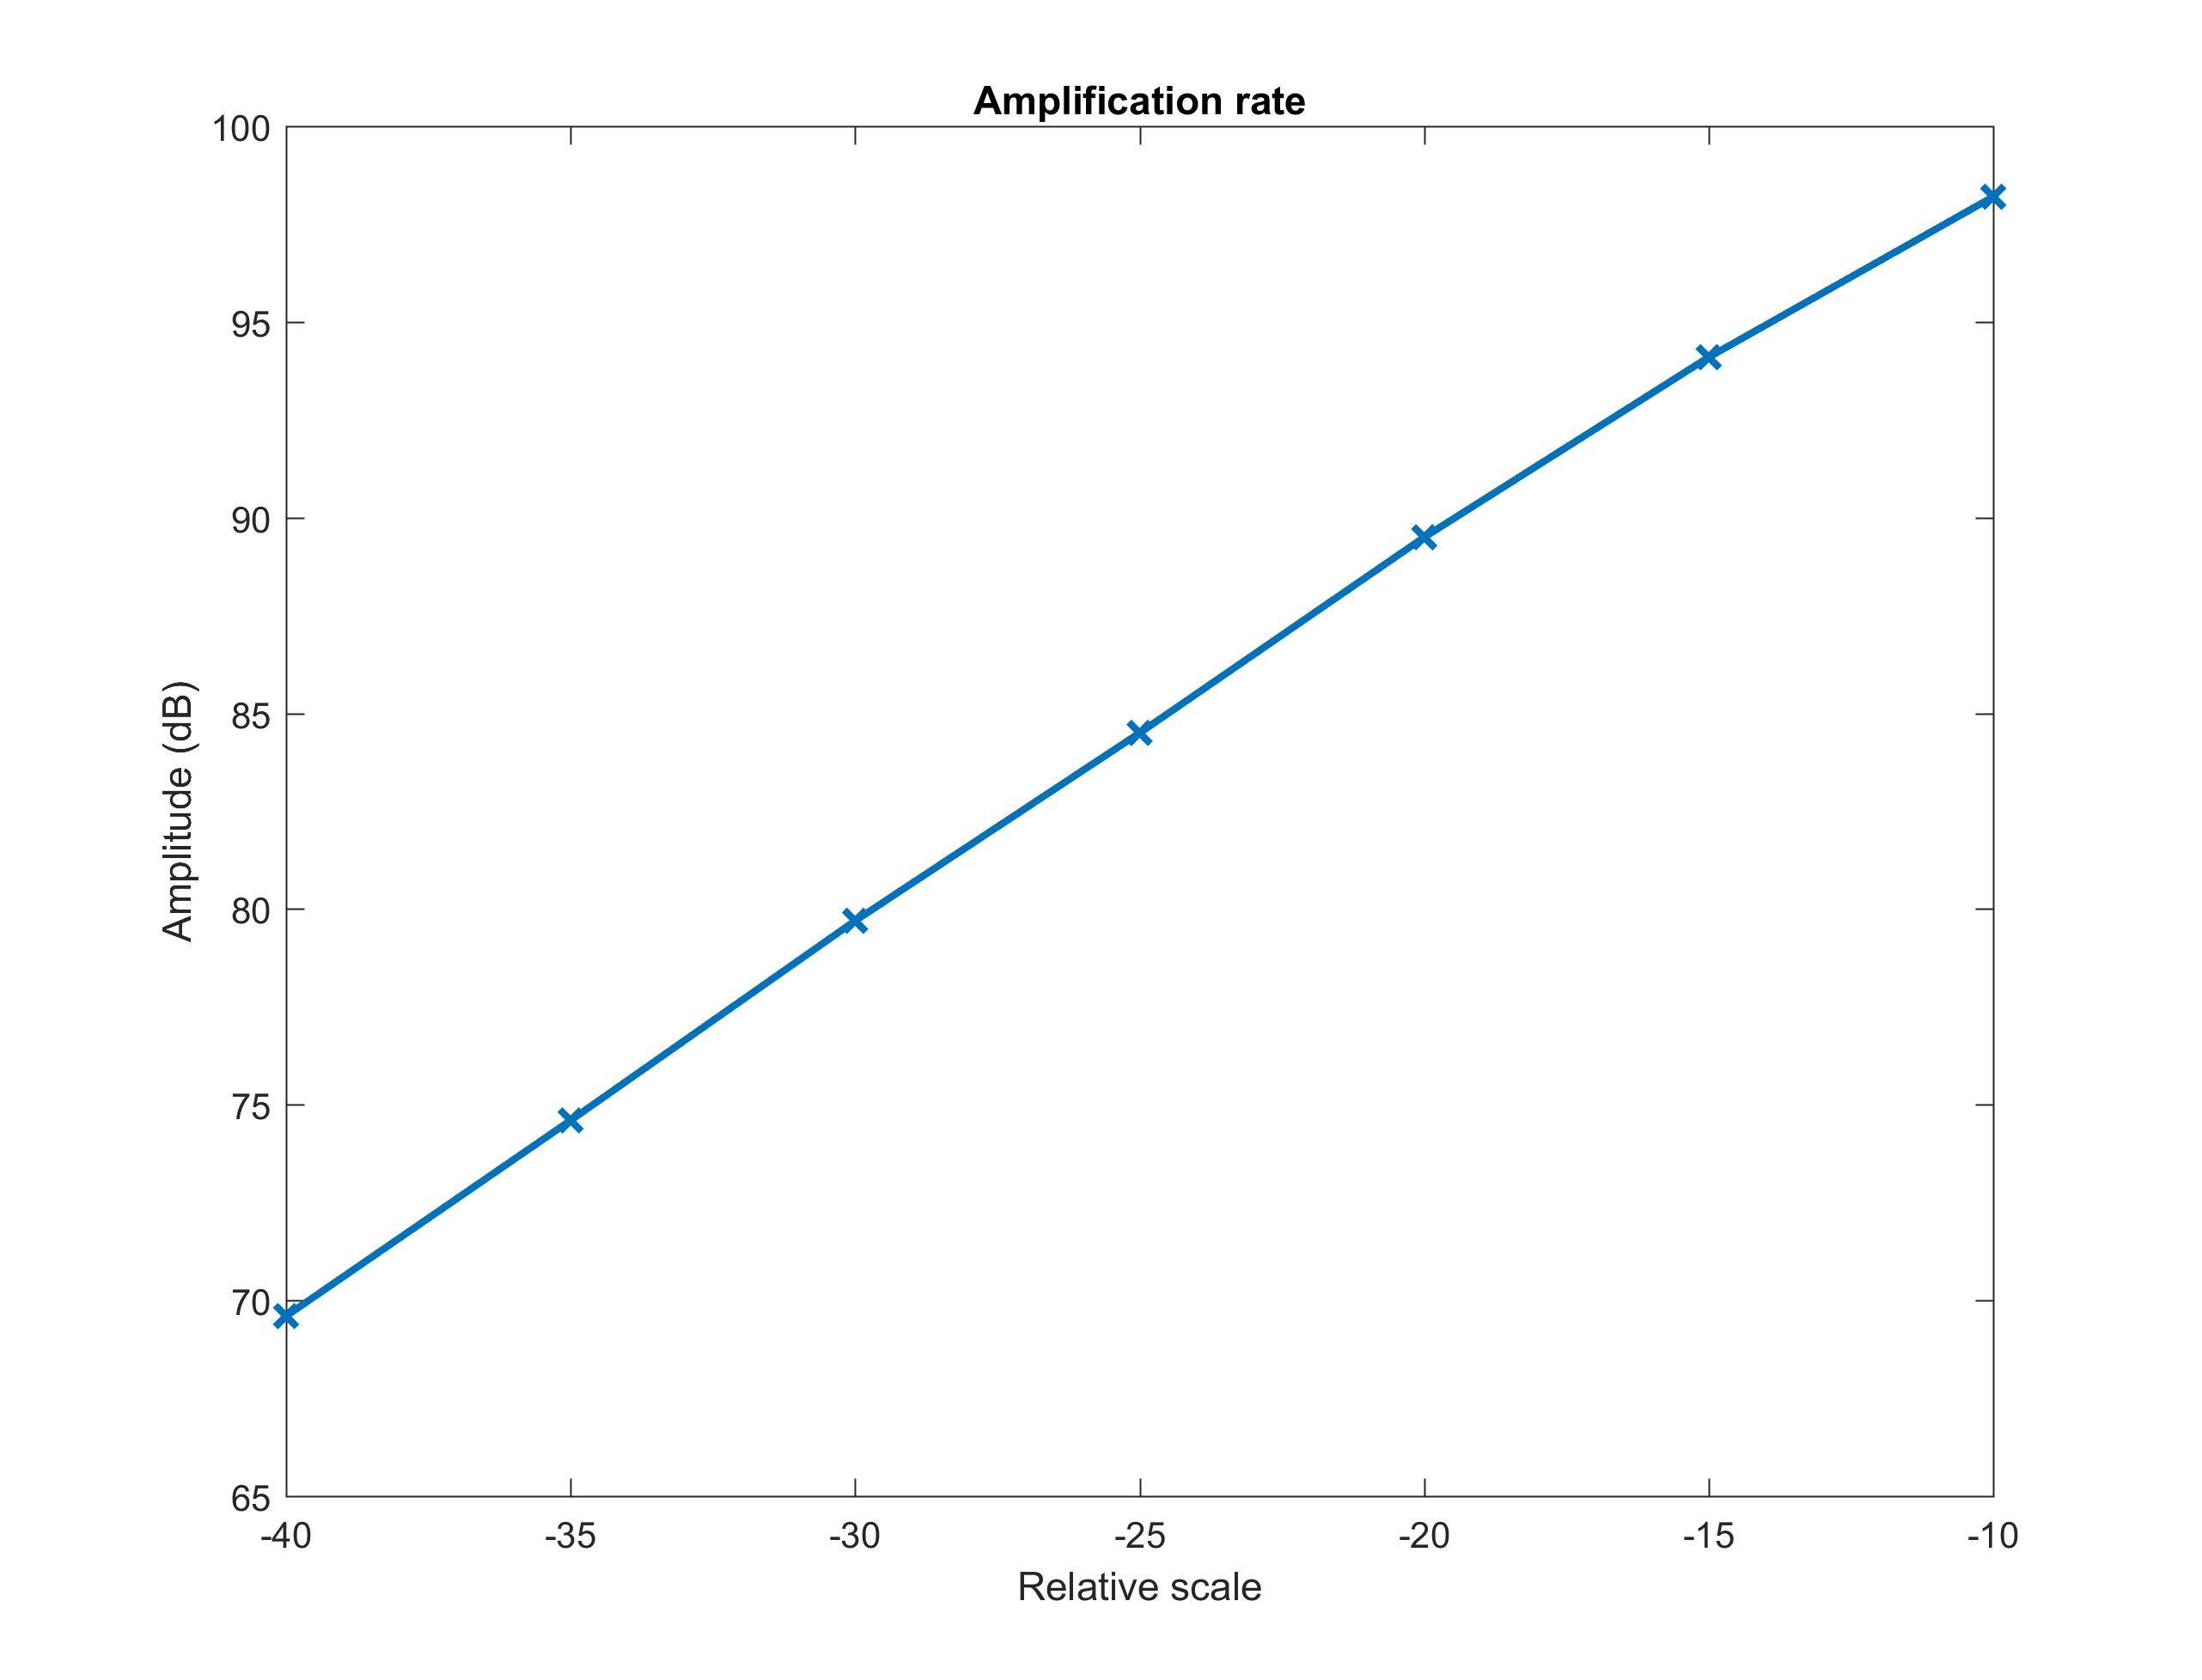
\includegraphics[width=13.5cm,height=13.5cm,keepaspectratio]{Figures/amplification}
\decoRule
\caption[Amplification factors]{Comparison between the relative scale and the corresponding SPL values.}
\label{fig:mics}
\end{figure}

All the results obtained using this set of loudspeakers will be represented using the relative scale above. When this is not the case the SPL level is specified together with position and model of the microphones used.
\\
The comparative study of the two models and the reasoning for the choosing of the SB speakers is described in section ~\ref{subsec:sbchoosing}.
\\
\\
Finally we have to measure the free field attenuation in the room, this is the value (in dB) that indicates how much the sound pressure decreases depending on the distance. This is the absolute lower minimum that we wish to increase with the ACC algorithm. By playing loudspeaker 22 (the rightmost of the one used in the center array in the anechoic chamber) we can measure an attenuation of \tld$2dB$ between the SPL measured in the bright zone versus the one measured in the dark zone. 

\subsection{Microphones}{}
\label{subsec:mics}

The microphones used for the experiments are of three kinds. The first and most used, situated inside the anechoic chamber are the Panasonic WM-61A, omnidirectional, condenser type microphones. They are pad-type circular instruments with a diameter of 0.6 cm. They draw their 2V at 500$\mu A$ of power from two custom made power supply units that are inside the anechoic chamber. The units are then connected to the A/D converters, outside the chamber.
\\
The microphones are soldered on top of a hollow metal rod, specifically made for the purpose, built using a CNC machine. The total diameter of the frame is $1$cm. The frequency range listed by the manufacturer is $50 - 15000$Hz with an impedance of $2.2$kOhm. Both the custom power suppliers and the microphone frame are property of the Aarhus University, made in the past years during other thesis projects.
\\
\\
the second kind is an NTi M2010 omnidirectional, condenser type, free field microphone. Its diameter is $5$cm and requires a phantom power supplier, positioned outside the anechoic chamber. It is connected to it through an XLR interface. the power supply is then connected to the A/D converter unit. This microphone was used for the nonlinear distortion estimation of the speakers.
\\
\\
The last kind are four Behringer ECM8000, omnidirectional, condenser type microphones. Those were used in the listening room. Those were connected to the Fireface UC unit, after being powered by two Millennium phantom power units.
\\
\\
All microphones have been calibrated prior use using a device that outputs a rated vaule of $1$Pa of sound pressure.

\subsubsection{Anechoic chamber setup}

The microphones are hold in place by a CNC carved, PMMA plastic (acrylic) frame bolted on a stand in a 6-by-8 configuration. The space between the microphones is hollowed in order to limit the reflections of the soundwaves at high frequencies. The distance between microphones (center-to-center) is $5$cm. The height of the matrix frame with the microphones is $111$cm (bottom-to-top), while the speaker array has a similar height, $108$cm from the floor to the center of the cones. The two controlled sound zones are symmetrically disposed at a longitudinal distance of $120$cm from the cones and $140$cm apart from each other. The center-to-center distance (the center of the microphone matrix versus the center of the middle speaker array) is $140$cm, which corresponds to an angle of \tld$29$ degrees.
\\
Due to limits in the available resources, there is only one microphone matrix available, even though there are two sound zones. This means that the instrumentation has to be moved between the two positions while performing the experiment (the experiment is repeated twice, once with the stand in the dark zone and one when in the bright zone).
\\
The microphone matrix is shown in figure ~\ref{fig:mics}.

\begin{figure}[H]
\centering
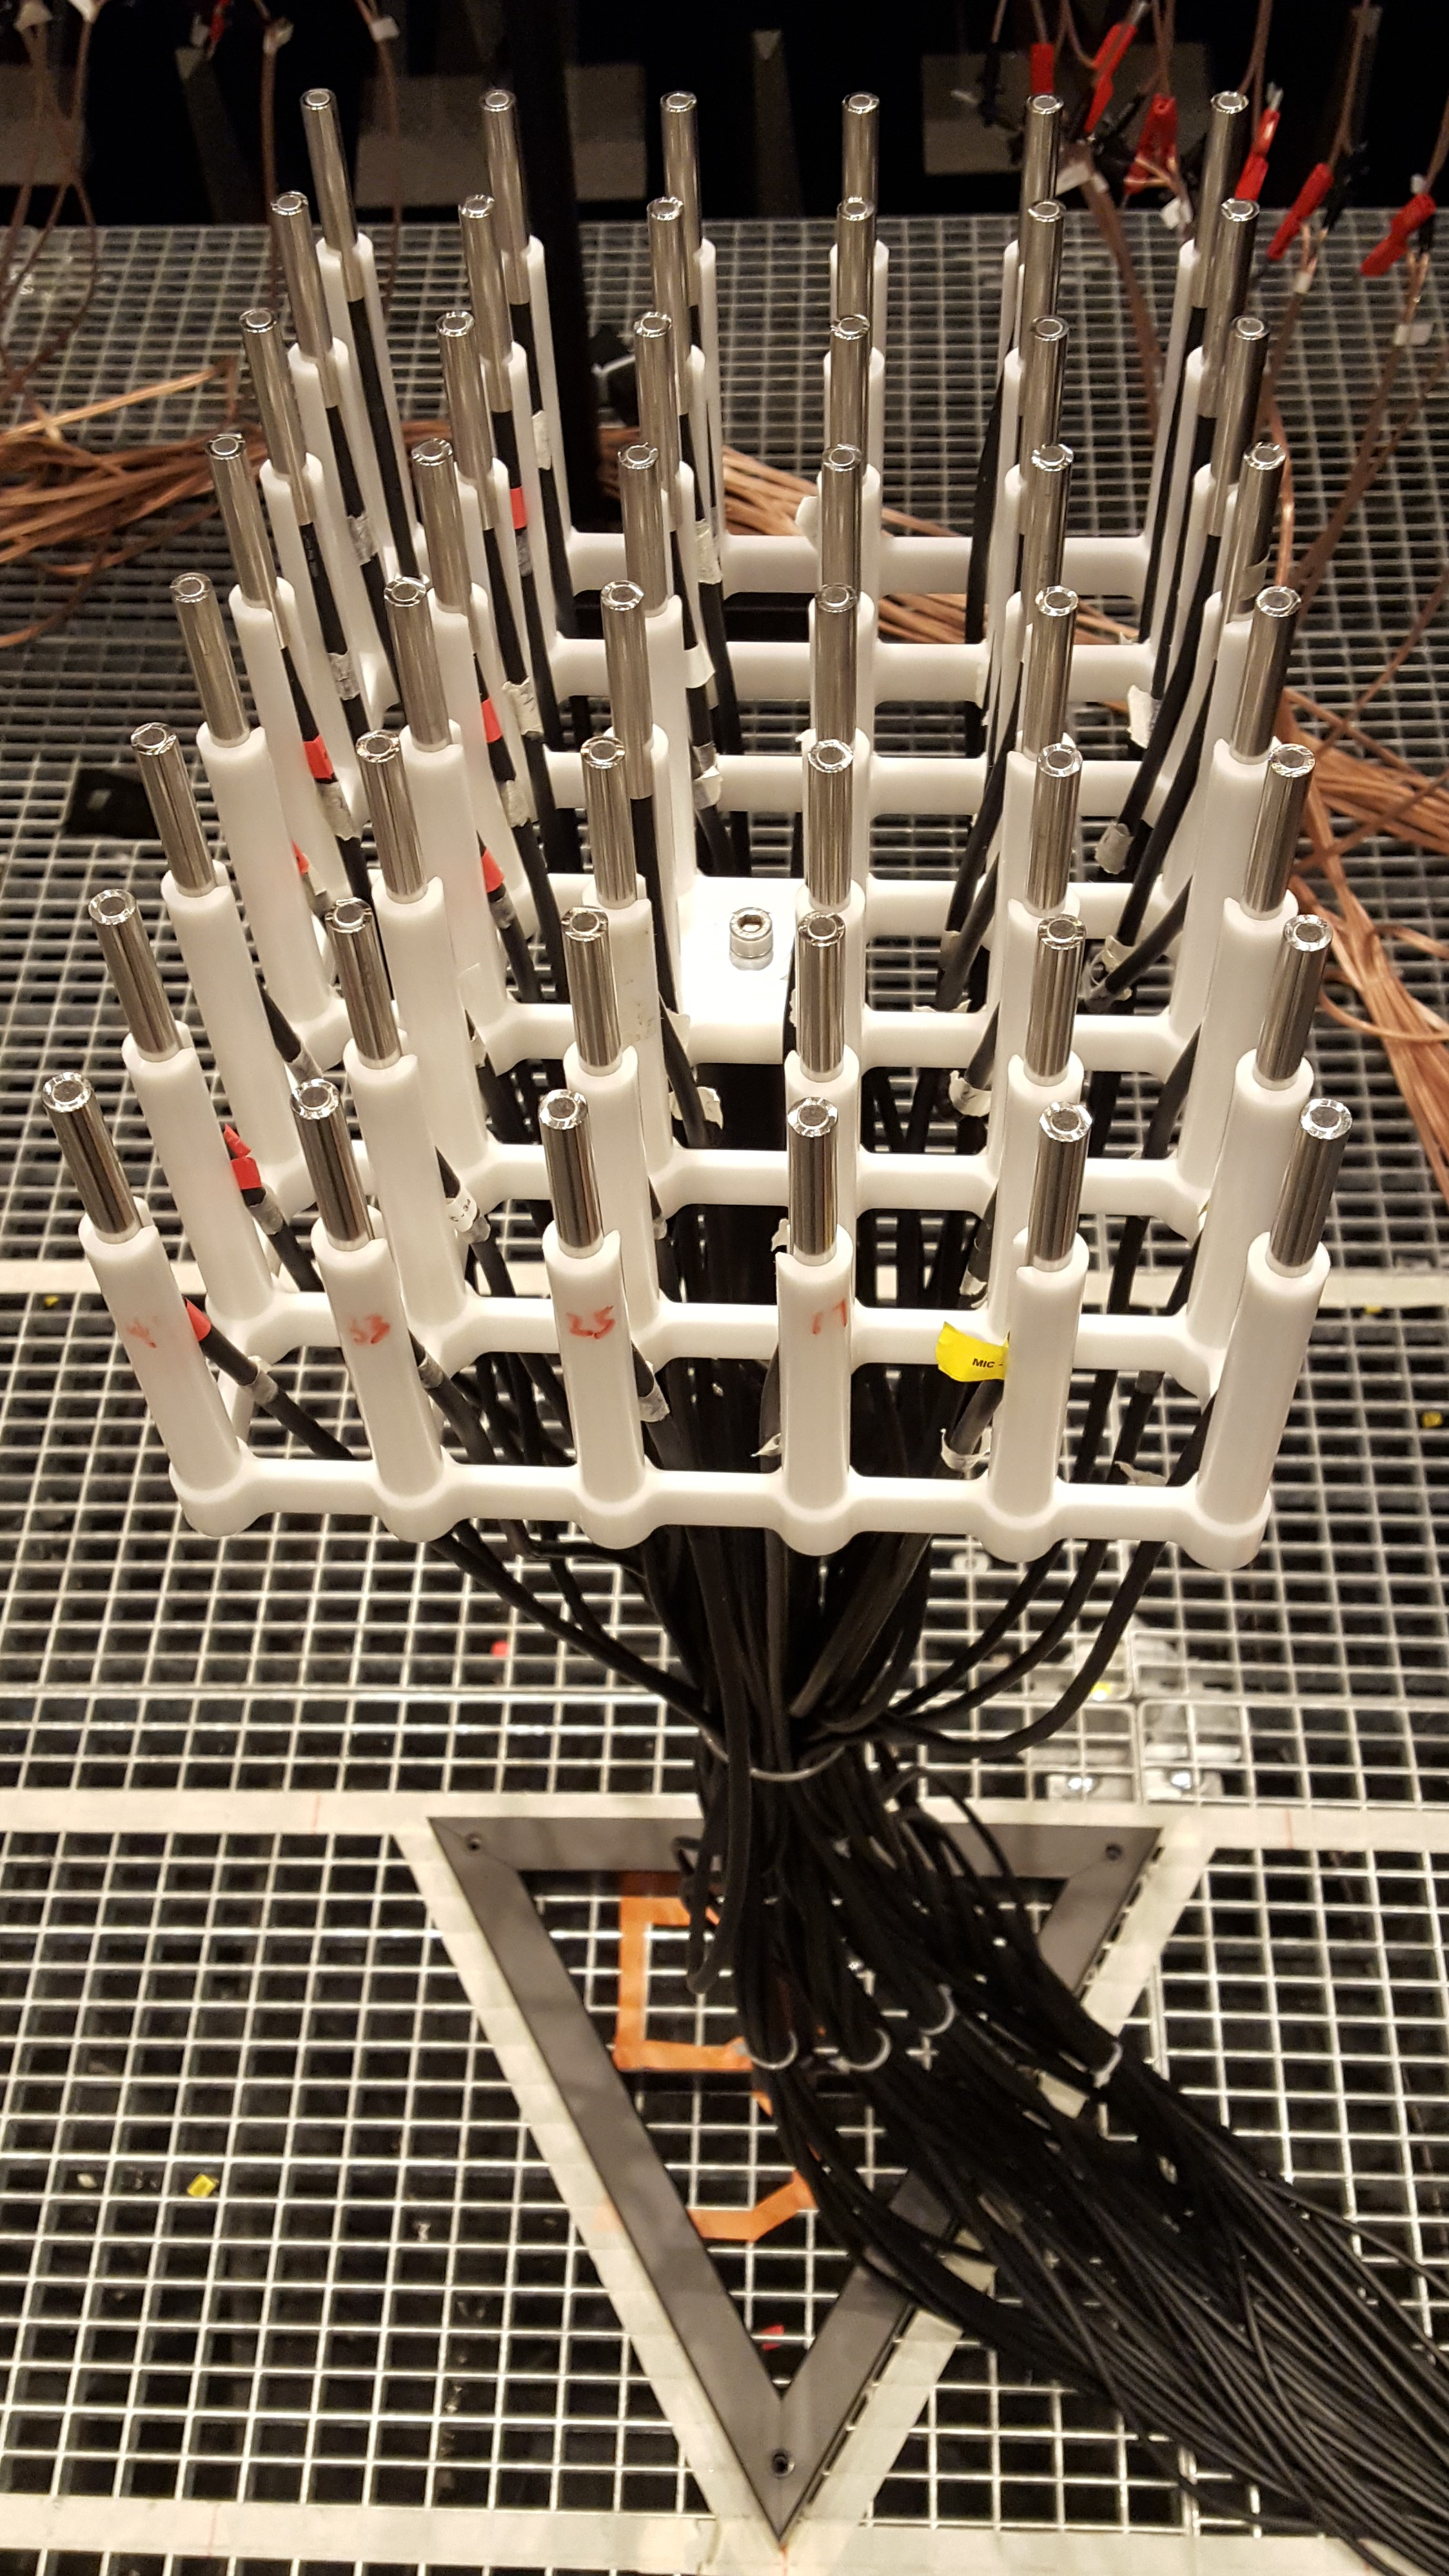
\includegraphics[width=10cm,height=10cm,keepaspectratio]{Figures/mics}
\decoRule
\caption[Microphone array with stand]{Microphone array with stand. the tape on the floor indicates the position of one of the two sound zones (the bright one in this case).}
\label{fig:mics}
\end{figure}

The distance between the microphones constitutes an higher limit to the sound frequencies that can be controlled. This is because of well known phenomenon of spatial aliasing, or grating.
\\
A soundwave should be sampled at more than two points per wavelength, otherwise the wave arrival direction becomes ambiguous. Having a distance $d$ of 5cm means that grating occurs at frequencies over $f = c/d \simeq 6.8$kHz, where c is the speed of sound ($343$ m/s in standard conditions). This value gives an ample security margin before the physical diameter of the microphones ($0.6 cm$) starts becoming a factor, in other words, the microphones can be considered detection points by the algorithm. 
\\
\\
Unfortunately, $6.8$kHz is not the upper limit before the grating effect appears. The relative angle between the center of the microphone matrix and the center of the loudspeakers array is another variable to take into account when defining the signal band. \parencite{cai_time-domain_2014} gives us the formula for the spacial aliasing, that is

\begin{equation}
f_{up}=\frac{c}{d(1+|sin \theta|)}
\label{eqn:freqaliasing}
\end{equation}

Where $c$ is the speed of sound, $d$ is the distance between the two centers and $\theta$ is their angle.
\\
Using the equation above, we find that $f_{up} \approx 2.9$kHz.
\\
\\
The SB speaker are divided in three arrays, each one having 12 driver units. The array at the center is the one used for the ACC experiments (speakers 13 to 24), while speakers 6 to 12 were briefly used for the experiment explained in section ~\ref{subsec:sbchoosing}. The central array was the one chosen for the experiments following the first one, because of its equal distance between the two sound zones, this causes a more balanced spread of the control effort undertaken by the single driver units.

\begin{figure}[H]
\centering
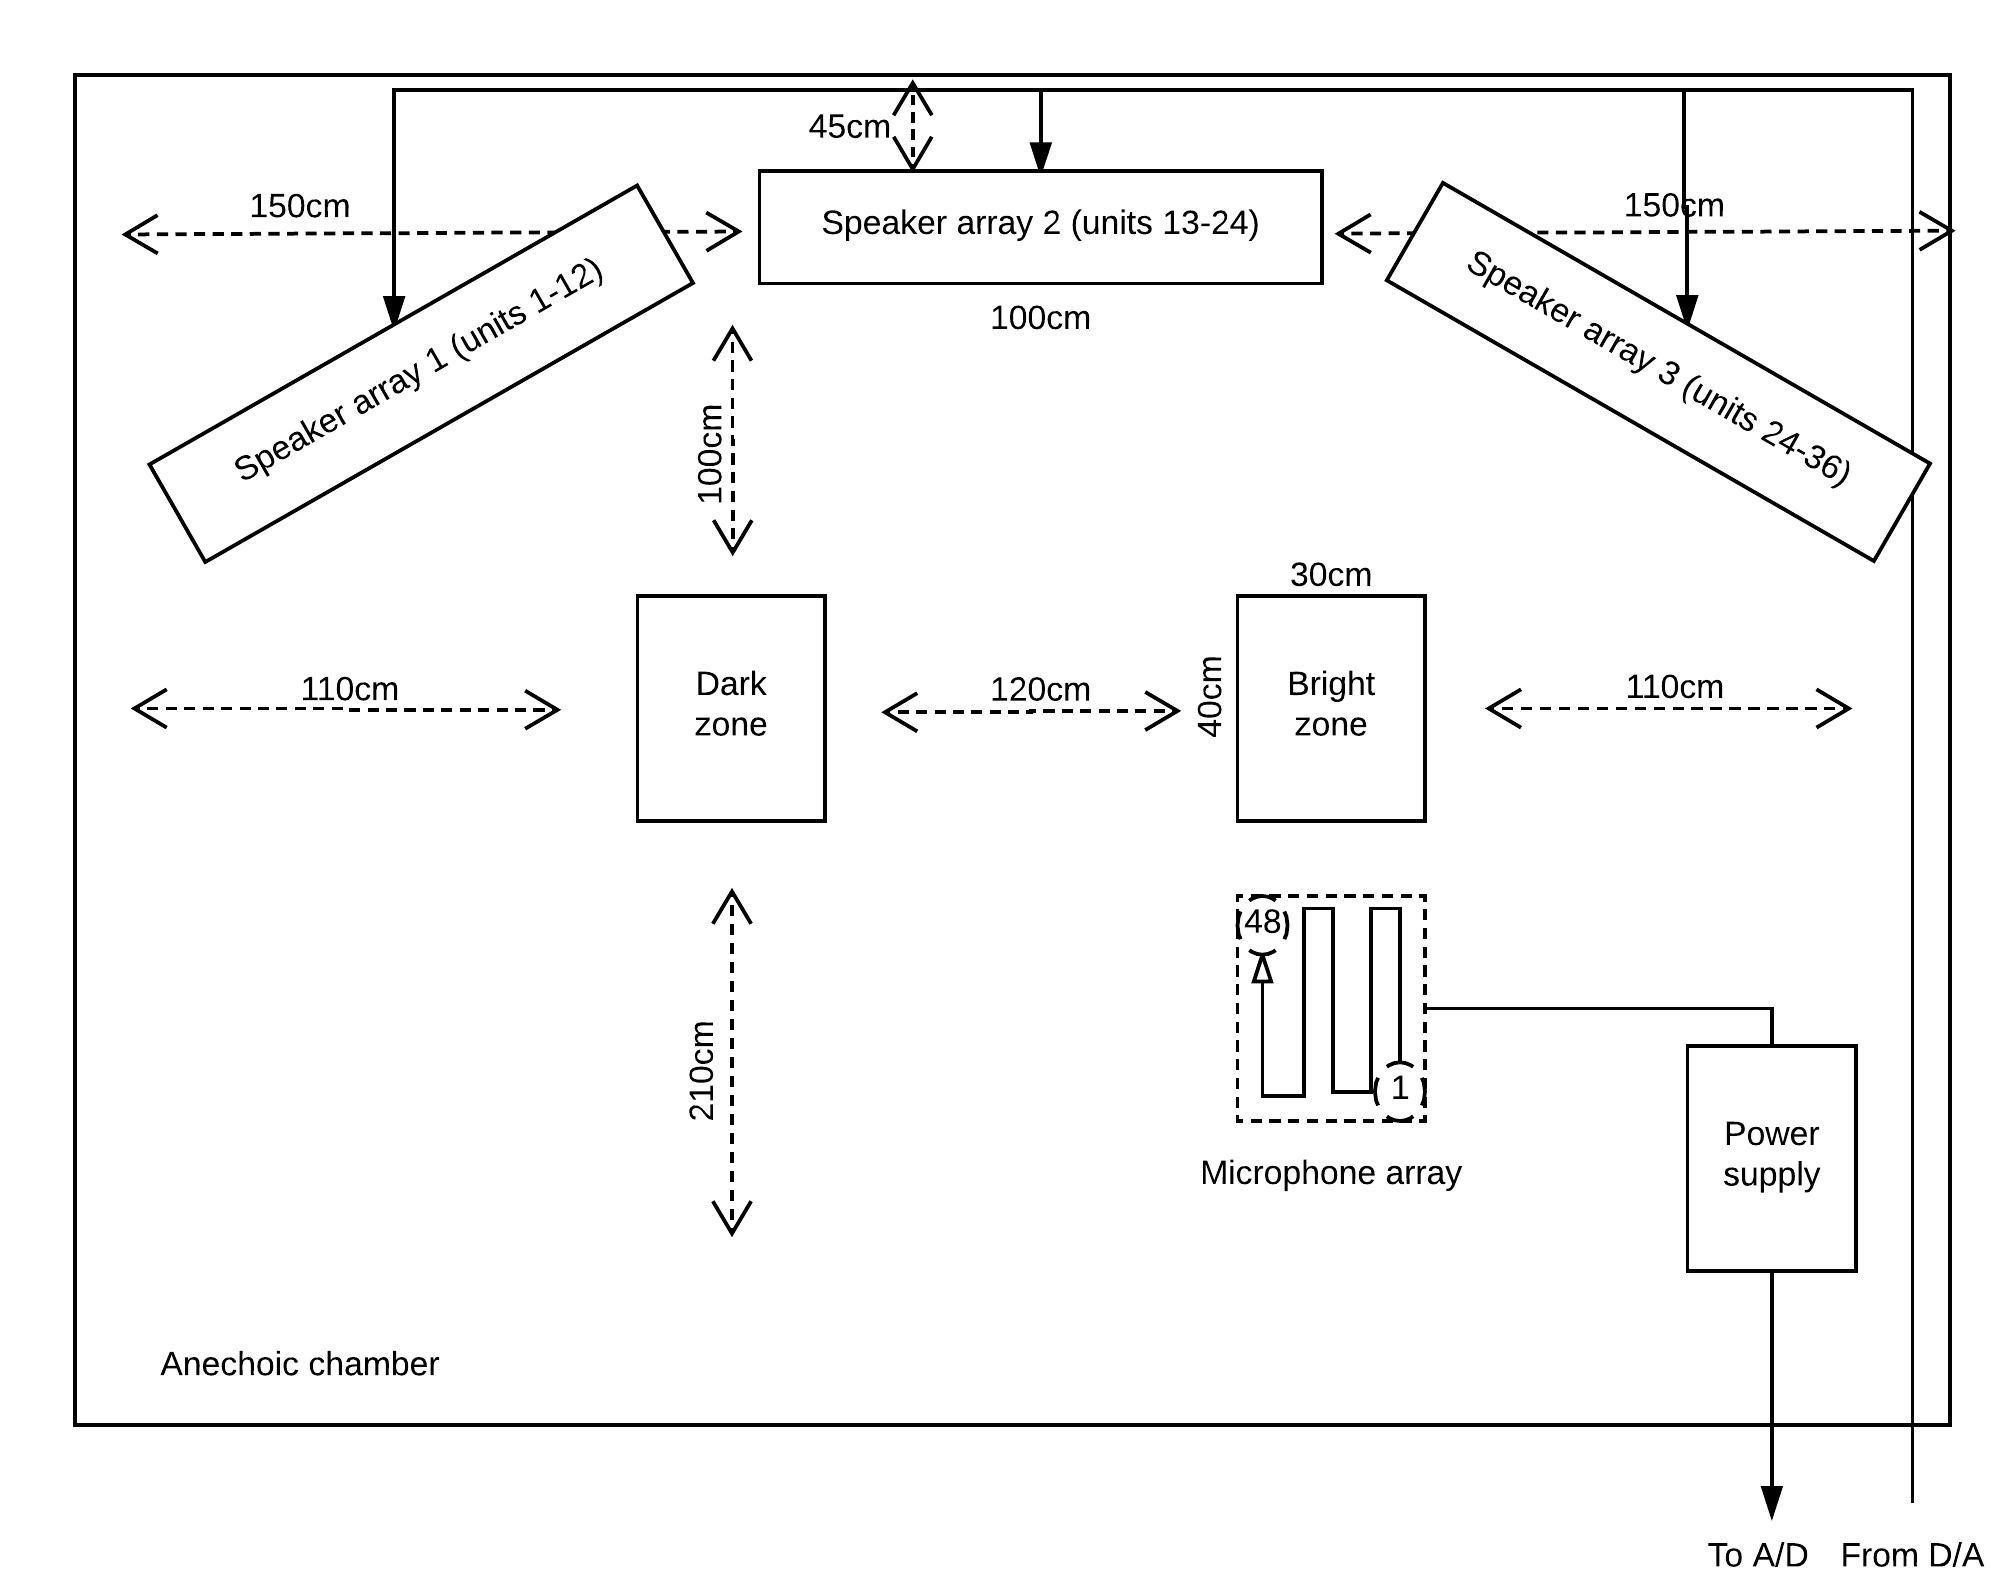
\includegraphics[width=14.5cm,height=15cm,keepaspectratio]{Figures/anechoicsetup}
\decoRule
\caption[Anechoic chamber setup]{The anechoic chamber setup.}
\label{fig:anechoicsetup}
\end{figure}

The presence of the other two arrays is justified by the fact that the room is also used for other experiments. The half-moon shape of the 3 arrays was chosen because the profile of the cabinets that causes reflections of the soundwaves is very limited. Since their impact in the contrast figure is minimal, it was not necessary to remove the units from the chamber.

\subsubsection{Listening room setup}

The microphones used in this scenario are mounted on a custom wooden frame, attached to a microphone stand. The microphones are positioned in circle. This was done to make sure they all had the same distance relative to each other.

\begin{figure}[H]
\centering
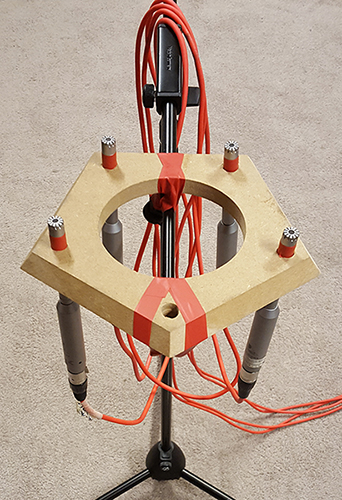
\includegraphics[width=8cm,height=8cm,keepaspectratio]{Figures/micslistening}
\decoRule
\caption[Microphone array in the listening room]{Microphone array with stand in the listening room.}
\label{fig:micslistening}
\end{figure}

In this case the frame has been carved out in the middle to limit the mechanical vibrations that high amplitude sounds might induce. Only four of the five microphone slots have been used, this is due hardware limitations in the input lines of the Fireface UC A/D converter.

\begin{figure}[H]
\centering
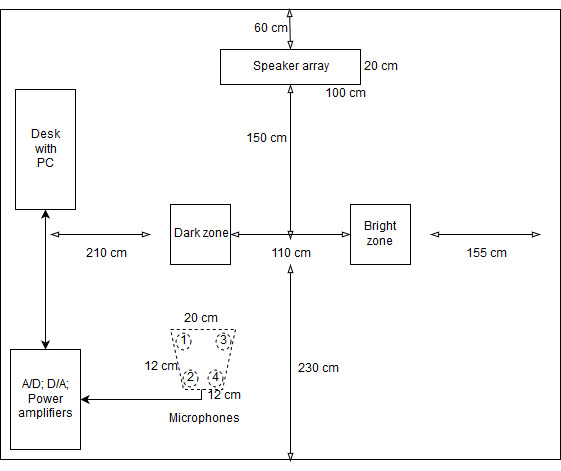
\includegraphics[width=13cm,height=12cm,keepaspectratio]{Figures/listeningsetup}
\decoRule
\caption[Listening room setup]{The listening room setup.}
\label{fig:listeningsetup}
\end{figure}

Finally, Using equation \ref{eqn:freqaliasing}, the upper frequency limit is $f_{up} \approx 3$kHz.

\subsection{Reflective surface}{}
\label{subsec:reflector}

The reflective surface used for the second part of the experiments is a plexiglass panel, mounted on a wooden frame. The panel dimensions are $125\textbf{x}105$cm (height and width), its thickness is $5.5$cm. The frame was realized by myself.

\begin{figure}[H]
\centering
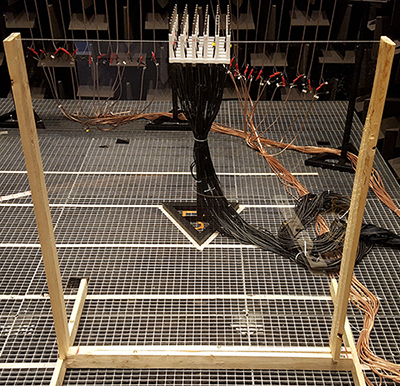
\includegraphics[width=8cm,height=8cm,keepaspectratio]{Figures/ref}
\decoRule
\caption[Reflective surface]{The reflective surface inside the room.}
\label{fig:refsurf}
\end{figure}

The reader will soon see how the introduction of the panel inside the anechoic chamber modifies the IR of the latter. By measuring the distance between the first peak, which corresponds to the arrival of the first, or "direct" sound to the microphones, and the second one, which marks the arrival of the reflected wave. 

\begin{figure}[H]
\centering
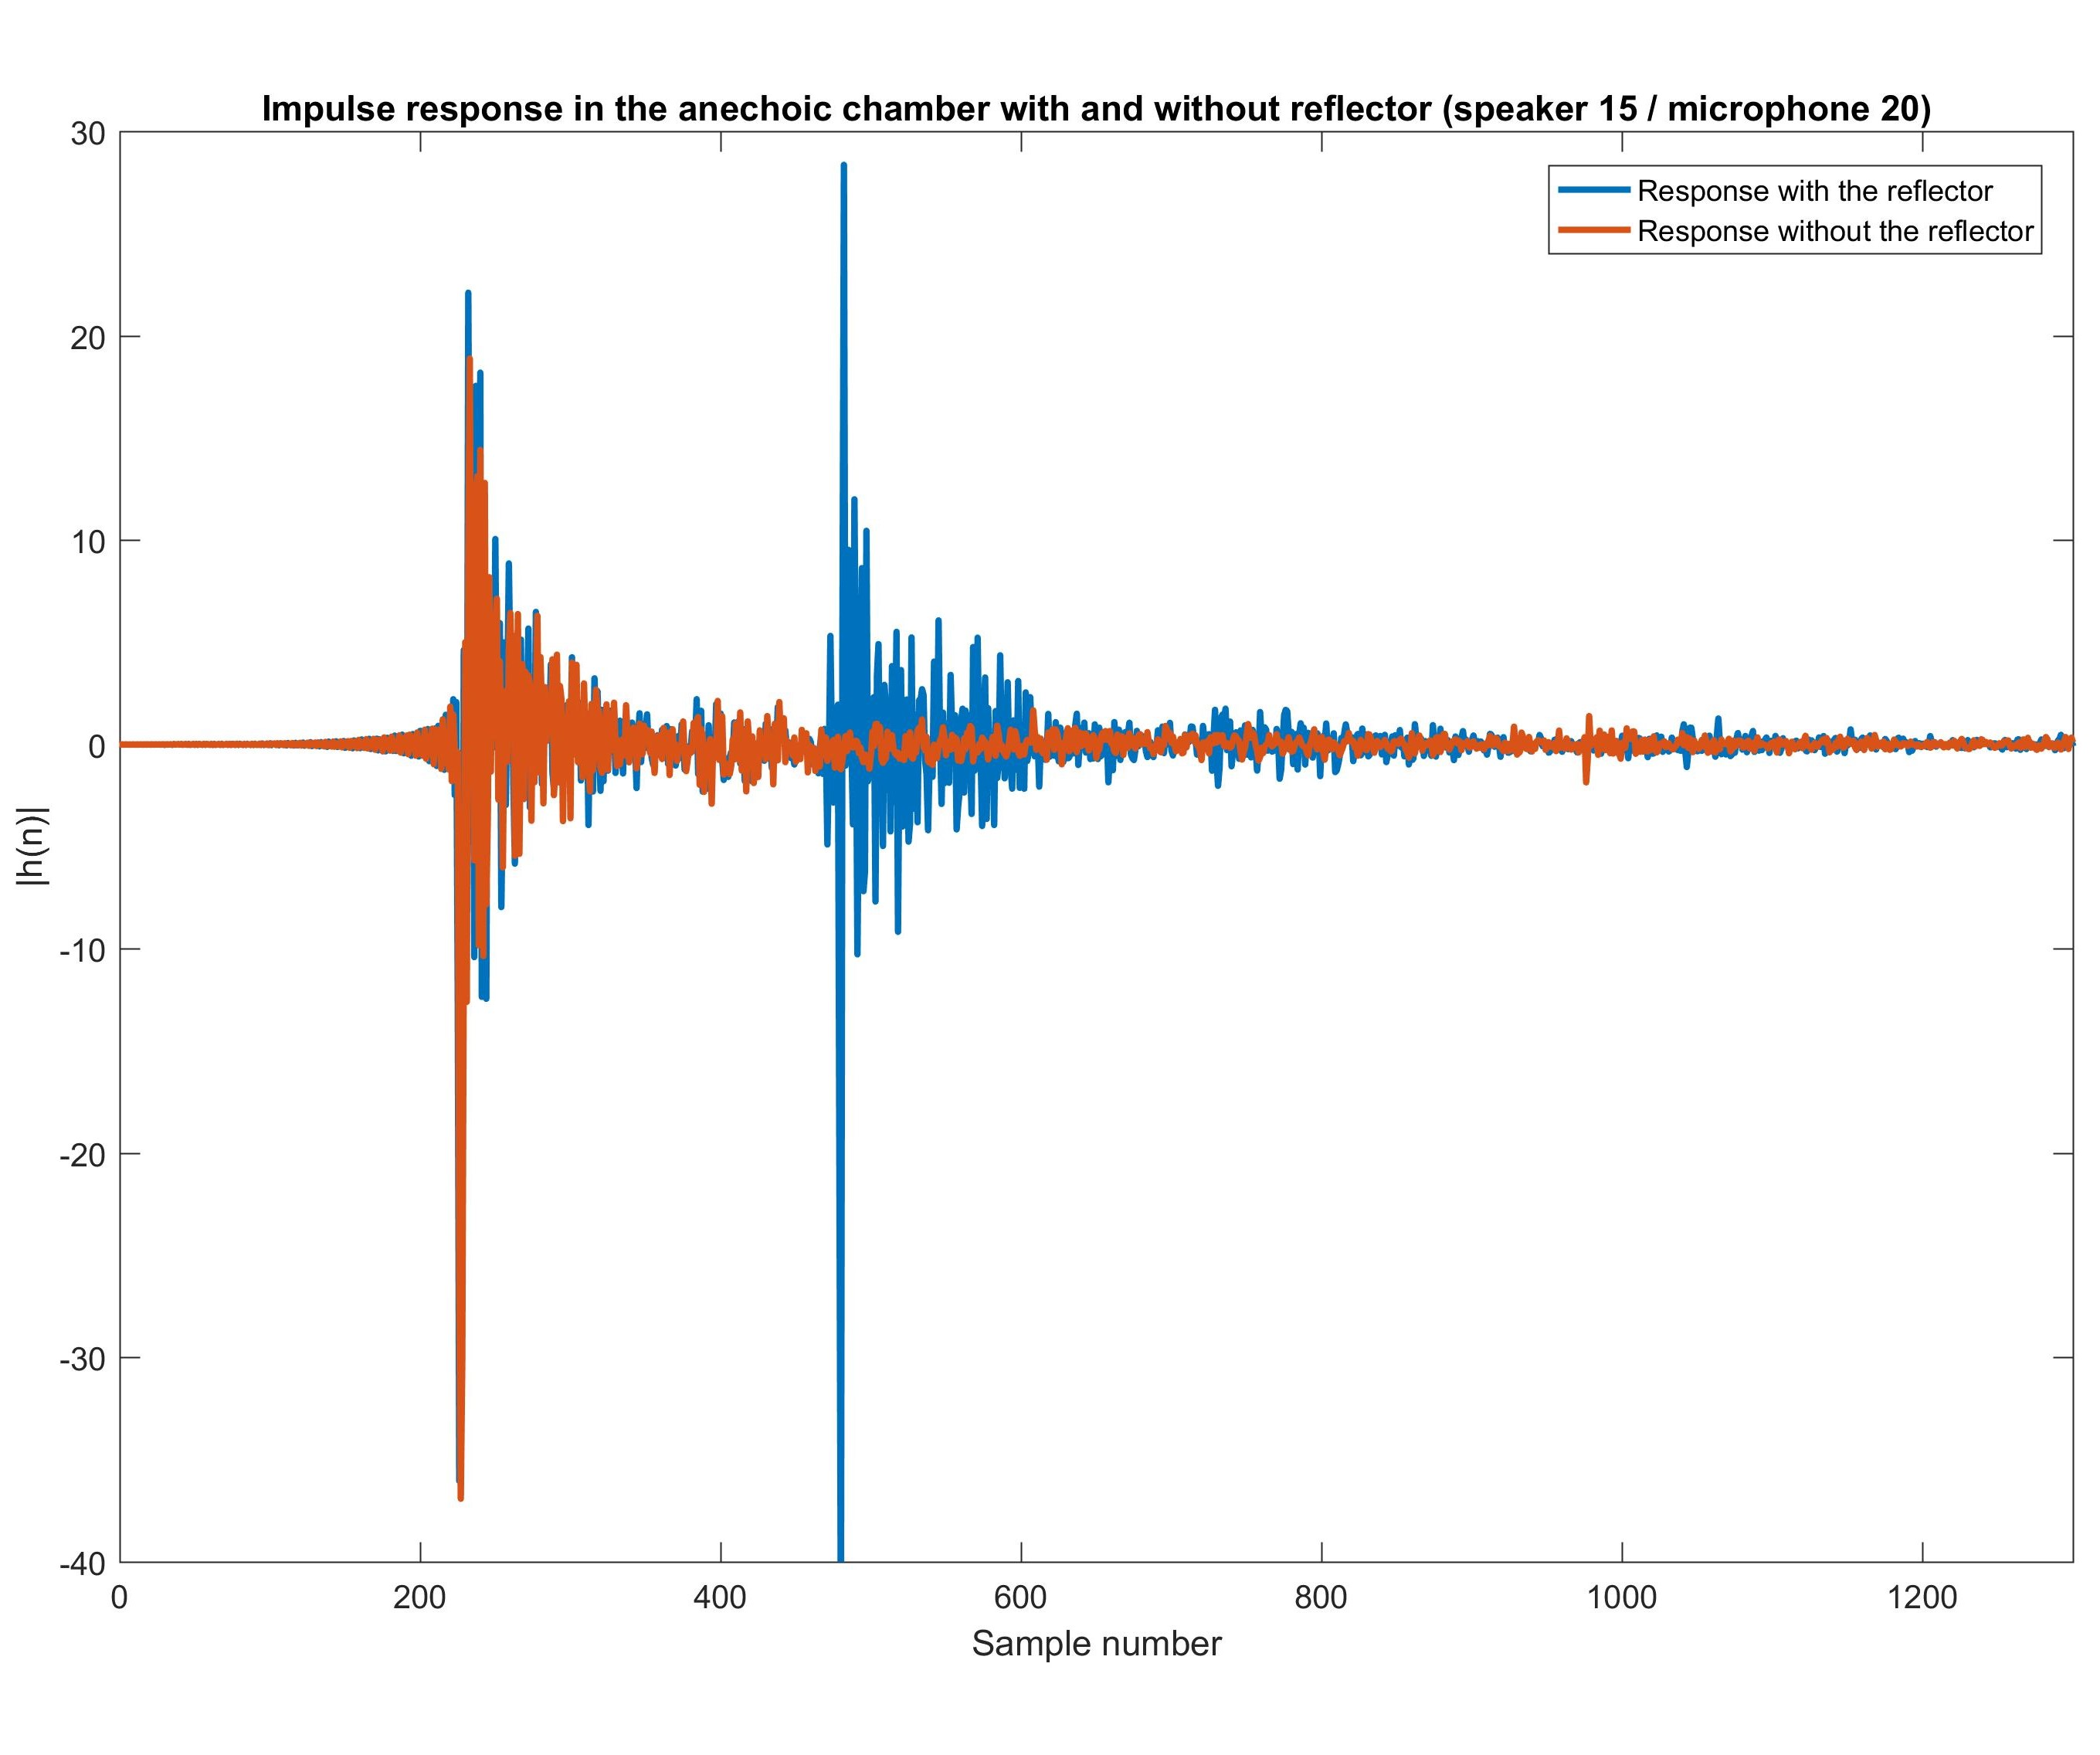
\includegraphics[width=14.5cm,height=15cm,keepaspectratio]{Figures/ir_ref_noref}
\decoRule
\caption[IR reflective surface]{Impulse response of the room when the panel is inside the room (blue line) compared to when it's not (orange line).}
\label{fig:irrefnoref}
\end{figure}

Please notice that the second peak has a bigger amplitude in the negative axis. This is because the direction of arrival of the reflection is opposite to the one of the direct wave.


\section{The signal chain}{}
\label{subsec:sigchain}

Once the desired digital signal is expressed in MATLAB and is sent to the computer's soundcard, by using the interfaces explained in section \ref{subsec:matlab}, it has to be converted in an analog signal, amplified and reproduced by the loudspeakers. In the meantime the resulting sound has to be recorded by the microphones.
\\
A schema representing the signal chain of the anechoic chamber is shown in Figure ~\ref{fig:signalchain}. Please notice that each box of the diagram represents an element where some kind of signal manipulation happens, like the conversion between digital, analog or mechanical domain. All the power amplifiers that, even tough scale the signal, do not change its domain, are omitted from the schema. In any case, both the loudspeakers and microphones are powered by such devices.

\begin{figure}[H]
\centering
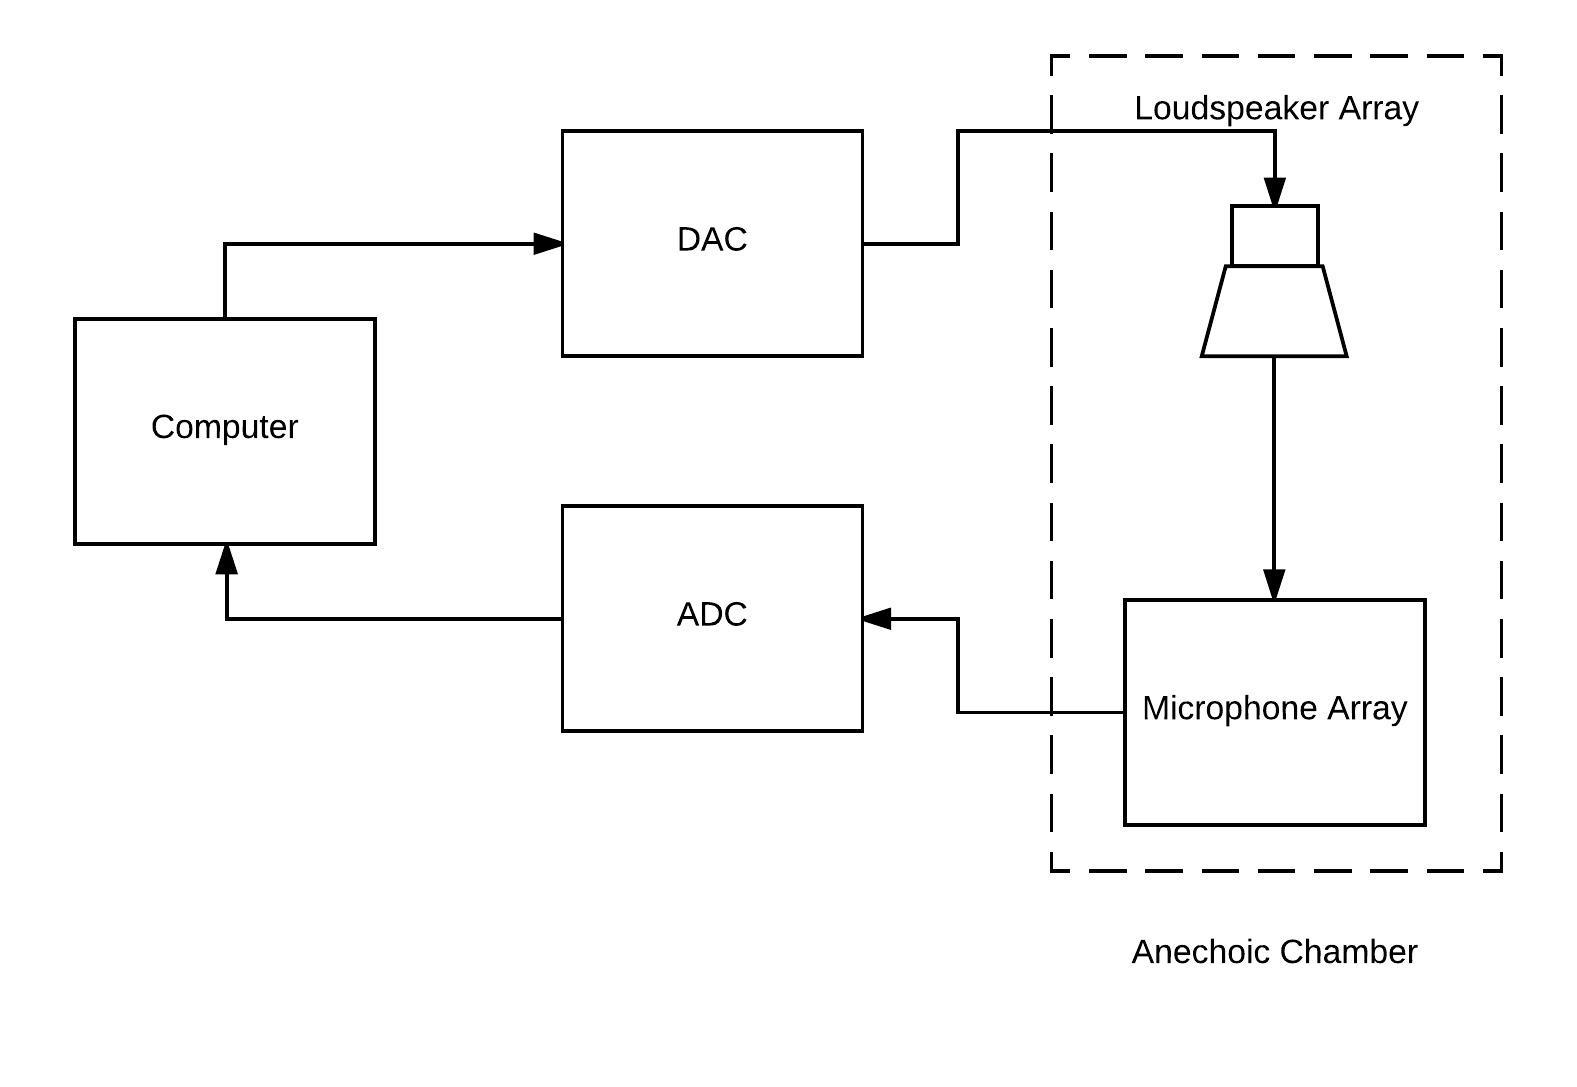
\includegraphics[width=12cm,height=12cm,keepaspectratio]{Figures/signalchain}
\decoRule
\caption[Signal Chain]{The signal chain.}
\label{fig:signalchain}
\end{figure}

The data lines for both the loudspeakers and the microphones are connected to the A/D converter units. One additional channel for both the elements is used for loopback. This means that they are not connected to an actual speaker or microphone, but rather they send data to the A/D input line, which mirrors it back to the computer trough its output lines. The purpose of this is to measure the delay that the converters introduce to the signal chain. Knowing this delay is very important, because it allows to synchronize the signal received form the microphones with the one sent out to the speakers. without it the filter calculated by the algorithm would not be convolved to the right samples, which means it would lose much of its effectiveness. Effectively, knowing this delay means that the first few samples recorded by the microphones have to be discarded. In most of the experiments run the loop delay is $\tld2200$ samples, with a sample rate of $48$kHz, which means it corresponds to $\tld0.046$s, which is in line with what can be reasonably expected by high quality of the instrumentation.
\\
\\
In the end, it has to be said that the signal chain in the listening room is identical to the one presented above, with the exception that all the instruments of the chain are situated inside the test room itself.
